
%% bare_conf.tex
%% V1.3
%% 2007/01/11
%% by Michael Shell
%% See:
%% http://www.michaelshell.org/
%% for current contact information.
%%
%% This is a skeleton file demonstrating the use of IEEEtran.cls
%% (requires IEEEtran.cls version 1.7 or later) with an IEEE conference paper.
%%
%% Support sites:
%% http://www.michaelshell.org/tex/ieeetran/
%% http://www.ctan.org/tex-archive/macros/latex/contrib/IEEEtran/
%% and
%% http://www.ieee.org/

%%*************************************************************************
%% Legal Notice:
%% This code is offered as-is without any warranty either expressed or
%% implied; without even the implied warranty of MERCHANTABILITY or
%% FITNESS FOR A PARTICULAR PURPOSE! 
%% User assumes all risk.
%% In no event shall IEEE or any contributor to this code be liable for
%% any damages or losses, including, but not limited to, incidental,
%% consequential, or any other damages, resulting from the use or misuse
%% of any information contained here.
%%
%% All comments are the opinions of their respective authors and are not
%% necessarily endorsed by the IEEE.
%%
%% This work is distributed under the LaTeX Project Public License (LPPL)
%% ( http://www.latex-project.org/ ) version 1.3, and may be freely used,
%% distributed and modified. A copy of the LPPL, version 1.3, is included
%% in the base LaTeX documentation of all distributions of LaTeX released
%% 2003/12/01 or later.
%% Retain all contribution notices and credits.
%% ** Modified files should be clearly indicated as such, including  **
%% ** renaming them and changing author support contact information. **
%%
%% File list of work: IEEEtran.cls, IEEEtran_HOWTO.pdf, bare_adv.tex,
%%                    bare_conf.tex, bare_jrnl.tex, bare_jrnl_compsoc.tex
%%*************************************************************************

% *** Authors should verify (and, if needed, correct) their LaTeX system  ***
% *** with the testflow diagnostic prior to trusting their LaTeX platform ***
% *** with production work. IEEE's font choices can trigger bugs that do  ***
% *** not appear when using other class files.                            ***
% The testflow support page is at:
% http://www.michaelshell.org/tex/testflow/



% Note that the a4paper option is mainly intended so that authors in
% countries using A4 can easily print to A4 and see how their papers will
% look in print - the typesetting of the document will not typically be
% affected with changes in paper size (but the bottom and side margins will).
% Use the testflow package mentioned above to verify correct handling of
% both paper sizes by the user's LaTeX system.
%
% Also note that the "draftcls" or "draftclsnofoot", not "draft", option
% should be used if it is desired that the figures are to be displayed in
% draft mode.
%
% \documentclass[10pt, conference, compsocconf]{IEEEtran}
\documentclass[conference,compsocconf]{IEEEtran}

% Add the compsocconf option for Computer Society conferences.
%
% If IEEEtran.cls has not been installed into the LaTeX system files,
% manually specify the path to it like:
% \documentclass[conference]{../sty/IEEEtran}





% Some very useful LaTeX packages include:
% (uncomment the ones you want to load)


% *** MISC UTILITY PACKAGES ***
%
%\usepackage{ifpdf}
% Heiko Oberdiek's ifpdf.sty is very useful if you need conditional
% compilation based on whether the output is pdf or dvi.
% usage:
% \ifpdf
%   % pdf code
% \else
%   % dvi code
% \fi
% The latest version of ifpdf.sty can be obtained from:
% http://www.ctan.org/tex-archive/macros/latex/contrib/oberdiek/
% Also, note that IEEEtran.cls V1.7 and later provides a builtin
% \ifCLASSINFOpdf conditional that works the same way.
% When switching from latex to pdflatex and vice-versa, the compiler may
% have to be run twice to clear warning/error messages.

\usepackage{amsmath,amssymb}

\usepackage[linesnumbered,boxed,ruled,vlined]{algorithm2e}
\usepackage[dvips]{graphicx}





% *** CITATION PACKAGES ***
%
\usepackage{cite}
% cite.sty was written by Donald Arseneau
% V1.6 and later of IEEEtran pre-defines the format of the cite.sty package
% \cite{} output to follow that of IEEE. Loading the cite package will
% result in citation numbers being automatically sorted and properly
% "compressed/ranged". e.g., [1], [9], [2], [7], [5], [6] without using
% cite.sty will become [1], [2], [5]--[7], [9] using cite.sty. cite.sty's
% \cite will automatically add leading space, if needed. Use cite.sty's
% noadjust option (cite.sty V3.8 and later) if you want to turn this off.
% cite.sty is already installed on most LaTeX systems. Be sure and use
% version 4.0 (2003-05-27) and later if using hyperref.sty. cite.sty does
% not currently provide for hyperlinked citations.
% The latest version can be obtained at:
% http://www.ctan.org/tex-archive/macros/latex/contrib/cite/
% The documentation is contained in the cite.sty file itself.






% *** GRAPHICS RELATED PACKAGES ***
%
\ifCLASSINFOpdf
  % \usepackage[pdftex]{graphicx}
  % declare the path(s) where your graphic files are
  % \graphicspath{{../pdf/}{../jpeg/}}
  % and their extensions so you won't have to specify these with
  % every instance of \includegraphics
  % \DeclareGraphicsExtensions{.pdf,.jpeg,.png}
\else
  % or other class option (dvipsone, dvipdf, if not using dvips). graphicx
  % will default to the driver specified in the system graphics.cfg if no
  % driver is specified.
  % \usepackage[dvips]{graphicx}
  % declare the path(s) where your graphic files are
  % \graphicspath{{../eps/}}
  % and their extensions so you won't have to specify these with
  % every instance of \includegraphics
  % \DeclareGraphicsExtensions{.eps}
\fi
% graphicx was written by David Carlisle and Sebastian Rahtz. It is
% required if you want graphics, photos, etc. graphicx.sty is already
% installed on most LaTeX systems. The latest version and documentation can
% be obtained at: 
% http://www.ctan.org/tex-archive/macros/latex/required/graphics/
% Another good source of documentation is "Using Imported Graphics in
% LaTeX2e" by Keith Reckdahl which can be found as epslatex.ps or
% epslatex.pdf at: http://www.ctan.org/tex-archive/info/
%
% latex, and pdflatex in dvi mode, support graphics in encapsulated
% postscript (.eps) format. pdflatex in pdf mode supports graphics
% in .pdf, .jpeg, .png and .mps (metapost) formats. Users should ensure
% that all non-photo figures use a vector format (.eps, .pdf, .mps) and
% not a bitmapped formats (.jpeg, .png). IEEE frowns on bitmapped formats
% which can result in "jaggedy"/blurry rendering of lines and letters as
% well as large increases in file sizes.
%
% You can find documentation about the pdfTeX application at:
% http://www.tug.org/applications/pdftex





% *** MATH PACKAGES ***
%
%\usepackage[cmex10]{amsmath}
% A popular package from the American Mathematical Society that provides
% many useful and powerful commands for dealing with mathematics. If using
% it, be sure to load this package with the cmex10 option to ensure that
% only type 1 fonts will utilized at all point sizes. Without this option,
% it is possible that some math symbols, particularly those within
% footnotes, will be rendered in bitmap form which will result in a
% document that can not be IEEE Xplore compliant!
%
% Also, note that the amsmath package sets \interdisplaylinepenalty to 10000
% thus preventing page breaks from occurring within multiline equations. Use:
%\interdisplaylinepenalty=2500
% after loading amsmath to restore such page breaks as IEEEtran.cls normally
% does. amsmath.sty is already installed on most LaTeX systems. The latest
% version and documentation can be obtained at:
% http://www.ctan.org/tex-archive/macros/latex/required/amslatex/math/





% *** SPECIALIZED LIST PACKAGES ***
%
%\usepackage{algorithmic}
% algorithmic.sty was written by Peter Williams and Rogerio Brito.
% This package provides an algorithmic environment fo describing algorithms.
% You can use the algorithmic environment in-text or within a figure
% environment to provide for a floating algorithm. Do NOT use the algorithm
% floating environment provided by algorithm.sty (by the same authors) or
% algorithm2e.sty (by Christophe Fiorio) as IEEE does not use dedicated
% algorithm float types and packages that provide these will not provide
% correct IEEE style captions. The latest version and documentation of
% algorithmic.sty can be obtained at:
% http://www.ctan.org/tex-archive/macros/latex/contrib/algorithms/
% There is also a support site at:
% http://algorithms.berlios.de/index.html
% Also of interest may be the (relatively newer and more customizable)
% algorithmicx.sty package by Szasz Janos:
% http://www.ctan.org/tex-archive/macros/latex/contrib/algorithmicx/




% *** ALIGNMENT PACKAGES ***
%
%\usepackage{array}
% Frank Mittelbach's and David Carlisle's array.sty patches and improves
% the standard LaTeX2e array and tabular environments to provide better
% appearance and additional user controls. As the default LaTeX2e table
% generation code is lacking to the point of almost being broken with
% respect to the quality of the end results, all users are strongly
% advised to use an enhanced (at the very least that provided by array.sty)
% set of table tools. array.sty is already installed on most systems. The
% latest version and documentation can be obtained at:
% http://www.ctan.org/tex-archive/macros/latex/required/tools/


%\usepackage{mdwmath}
%\usepackage{mdwtab}
% Also highly recommended is Mark Wooding's extremely powerful MDW tools,
% especially mdwmath.sty and mdwtab.sty which are used to format equations
% and tables, respectively. The MDWtools set is already installed on most
% LaTeX systems. The lastest version and documentation is available at:
% http://www.ctan.org/tex-archive/macros/latex/contrib/mdwtools/


% IEEEtran contains the IEEEeqnarray family of commands that can be used to
% generate multiline equations as well as matrices, tables, etc., of high
% quality.


%\usepackage{eqparbox}
% Also of notable interest is Scott Pakin's eqparbox package for creating
% (automatically sized) equal width boxes - aka "natural width parboxes".
% Available at:
% http://www.ctan.org/tex-archive/macros/latex/contrib/eqparbox/





% *** SUBFIGURE PACKAGES ***
%\usepackage[tight,footnotesize]{subfigure}
% subfigure.sty was written by Steven Douglas Cochran. This package makes it
% easy to put subfigures in your figures. e.g., "Figure 1a and 1b". For IEEE
% work, it is a good idea to load it with the tight package option to reduce
% the amount of white space around the subfigures. subfigure.sty is already
% installed on most LaTeX systems. The latest version and documentation can
% be obtained at:
% http://www.ctan.org/tex-archive/obsolete/macros/latex/contrib/subfigure/
% subfigure.sty has been superceeded by subfig.sty.



%\usepackage[caption=false]{caption}
%\usepackage[font=footnotesize]{subfig}
% subfig.sty, also written by Steven Douglas Cochran, is the modern
% replacement for subfigure.sty. However, subfig.sty requires and
% automatically loads Axel Sommerfeldt's caption.sty which will override
% IEEEtran.cls handling of captions and this will result in nonIEEE style
% figure/table captions. To prevent this problem, be sure and preload
% caption.sty with its "caption=false" package option. This is will preserve
% IEEEtran.cls handing of captions. Version 1.3 (2005/06/28) and later 
% (recommended due to many improvements over 1.2) of subfig.sty supports
% the caption=false option directly:
%\usepackage[caption=false,font=footnotesize]{subfig}
%
% The latest version and documentation can be obtained at:
% http://www.ctan.org/tex-archive/macros/latex/contrib/subfig/
% The latest version and documentation of caption.sty can be obtained at:
% http://www.ctan.org/tex-archive/macros/latex/contrib/caption/




% *** FLOAT PACKAGES ***
%
%\usepackage{fixltx2e}
% fixltx2e, the successor to the earlier fix2col.sty, was written by
% Frank Mittelbach and David Carlisle. This package corrects a few problems
% in the LaTeX2e kernel, the most notable of which is that in current
% LaTeX2e releases, the ordering of single and double column floats is not
% guaranteed to be preserved. Thus, an unpatched LaTeX2e can allow a
% single column figure to be placed prior to an earlier double column
% figure. The latest version and documentation can be found at:
% http://www.ctan.org/tex-archive/macros/latex/base/



%\usepackage{stfloats}
% stfloats.sty was written by Sigitas Tolusis. This package gives LaTeX2e
% the ability to do double column floats at the bottom of the page as well
% as the top. (e.g., "\begin{figure*}[!b]" is not normally possible in
% LaTeX2e). It also provides a command:
%\fnbelowfloat
% to enable the placement of footnotes below bottom floats (the standard
% LaTeX2e kernel puts them above bottom floats). This is an invasive package
% which rewrites many portions of the LaTeX2e float routines. It may not work
% with other packages that modify the LaTeX2e float routines. The latest
% version and documentation can be obtained at:
% http://www.ctan.org/tex-archive/macros/latex/contrib/sttools/
% Documentation is contained in the stfloats.sty comments as well as in the
% presfull.pdf file. Do not use the stfloats baselinefloat ability as IEEE
% does not allow \baselineskip to stretch. Authors submitting work to the
% IEEE should note that IEEE rarely uses double column equations and
% that authors should try to avoid such use. Do not be tempted to use the
% cuted.sty or midfloat.sty packages (also by Sigitas Tolusis) as IEEE does
% not format its papers in such ways.





% *** PDF, URL AND HYPERLINK PACKAGES ***
%
%\usepackage{url}
% url.sty was written by Donald Arseneau. It provides better support for
% handling and breaking URLs. url.sty is already installed on most LaTeX
% systems. The latest version can be obtained at:
% http://www.ctan.org/tex-archive/macros/latex/contrib/misc/
% Read the url.sty source comments for usage information. Basically,
% \url{my_url_here}.





% *** Do not adjust lengths that control margins, column widths, etc. ***
% *** Do not use packages that alter fonts (such as pslatex).         ***
% There should be no need to do such things with IEEEtran.cls V1.6 and later.
% (Unless specifically asked to do so by the journal or conference you plan
% to submit to, of course. )


% correct bad hyphenation here
\hyphenation{op-tical net-works semi-conduc-tor}

\newtheorem{theorem}{\textbf{Theorem}} 

\newtheorem{definition}{\textbf{Definition}} 

\newtheorem{lemma}{\textbf{Lemma}} 

\newtheorem{Procedure}{\textbf{Procedure}} 

\newtheorem{inference}{\textbf{Inference}} 



\begin{document}
%
% paper title
% can use linebreaks \\ within to get better formatting as desired
\title{Structure-Aware CNF Obfuscation for Privacy-Preserving SAT Solving}


% author names and affiliations
% use a multiple column layout for up to two different
% affiliations

\author{
\IEEEauthorblockN{Ying Qin\IEEEauthorrefmark{1},
ShengYu Shen\IEEEauthorrefmark{1} and
Yan Jia\IEEEauthorrefmark{1}
}
\IEEEauthorblockA{
\IEEEauthorrefmark{1}College of computer\\
National University of Defense Technology,
ChangSha, China 410073\\ 
Email: \{yingqin,syshen,yjia\}@nudt.edu.cn
}
}
% conference papers do not typically use \thanks and this command
% is locked out in conference mode. If really needed, such as for
% the acknowledgment of grants, issue a \IEEEoverridecommandlockouts
% after \documentclass

% for over three affiliations, or if they all won't fit within the width
% of the page, use this alternative format:
% 
%\author{\IEEEauthorblockN{Michael Shell\IEEEauthorrefmark{1},
%Homer Simpson\IEEEauthorrefmark{2},
%James Kirk\IEEEauthorrefmark{3}, 
%Montgomery Scott\IEEEauthorrefmark{3} and
%Eldon Tyrell\IEEEauthorrefmark{4}}
%\IEEEauthorblockA{\IEEEauthorrefmark{1}School of Electrical and Computer Engineering\\
%Georgia Institute of Technology,
%Atlanta, Georgia 30332--0250\\ Email: see http://www.michaelshell.org/contact.html}
%\IEEEauthorblockA{\IEEEauthorrefmark{2}Twentieth Century Fox, Springfield, USA\\
%Email: homer@thesimpsons.com}
%\IEEEauthorblockA{\IEEEauthorrefmark{3}Starfleet Academy, San Francisco, California 96678-2391\\
%Telephone: (800) 555--1212, Fax: (888) 555--1212}
%\IEEEauthorblockA{\IEEEauthorrefmark{4}Tyrell Inc., 123 Replicant Street, Los Angeles, California 90210--4321}}




% use for special paper notices
%\IEEEspecialpapernotice{(Invited Paper)}




% make the title area
\maketitle


\begin{abstract}
In this paper, we study the problem of solving hard propositional satisfiability problem in Cloud or computing grid,
which is honest-but-curious.
We propose an approach to preserve input and output privacy based on CNF obfuscation,
and present obfuscation algorithm and its corresponding solution recovery algorithm.
By obfuscation, the CNF formula is transformed into another formula,
with different circuit structure and over-approximated solution space.
Solution of the original CNF can be extracted from the solution of obfuscated CNF by solution recovery.
Theoretical analysis demonstrates that,
obfuscation algorithm can significantly change the structure of CNF formula with polynomial time complexity,
while solution recovery algorithm can filter out solution with linear time complexity.
Experimental results on ISCAS89 benchmark show that obfuscation incurs acceptable negative impact on the performance of SAT solving.
\end{abstract}

\begin{IEEEkeywords}
component; formatting; style; styling;

\end{IEEEkeywords}


% For peer review papers, you can put extra information on the cover
% page as needed:
% \ifCLASSOPTIONpeerreview
% \begin{center} \bfseries EDICS Category: 3-BBND \end{center}
% \fi
%
% For peerreview papers, this IEEEtran command inserts a page break and
% creates the second title. It will be ignored for other modes.
\IEEEpeerreviewmaketitle



\section{Introduction}
% no \IEEEPARstart
Propositional satisfiability\cite{SATtheory} has been widely used in hardware and software verification\cite{HardwareSAT,softwareSAT},
cryptography\cite{cryptoSAT} etc.
With the rapid increase of the hardware and software system size,
the size of SAT problem generated from verification  also increases rapidly.
On the other hand, Cloud and grid can provide elastic computing resource,
which make outsourcing hard SAT problem to public Cloud or computation grid\cite{Nordugrid,CloudSMT,OneSpin} very attractive.

However, security issues make many customers reluctant to move their critical computation tasks to grid or Cloud.
Since the grid is constructed by loosely connecting a large number of readily available, high-end, heterogeneous computing facilities\cite{Nordugrid},
the risks posed by hoarding participants in grid computing environments are real and immediate\cite{HV-grid}.
While the Cloud vendors can be trusted and the Cloud infrastructure (i.e., the virtualization layer) can be assumed to be secure,
the virtual machines cannot be trusted to be always honest and loyal.
Literature\cite{AMI} points out security vulnerability that Amazon EC2 suffered from: 
Since Amazon Machine Image (AMI) are widely shared among the EC2 community,
a malicious AMI could flood the community with hundreds of infected virtual instances.
Literature \cite{InformationLeakageofCloud} also points out
the possibility of attacking virtual machine
through another virtual machine in the same physical machine.

These facts show that input and output data of SAT problem may be exposed to untrusted third party,
who may inspect valuable information from these data.
For example, SAT program originated from verification may suffer from leakage of privacy, such as circuit structure information.
Works carried out by Roy\cite{csRoy} and Fu \cite{csFu} suggest the possibility of extracting circuit information from CNF formula.
Furthermore, Du\cite{HV-grid} called solution of hard SAT problem generating from cryptograph etc as high-value rare events, 
and point out that the solution of SAT problem should also be treated as privacy, 
because it may be leaked to third party by hoarding participants.
Moreover, the SAT solver deployed in grid or Cloud may also be compromised by adversary, 
who may compel SAT solver to return incorrect result to  mislead verification.

These threats put customers who plan to outsource SAT solving in a dilemma:
using public Cloud or grid in open environment is cost-efficiently, 
but may suffer from leakage of privacy or incorrect result.
In order to meet this challenge, we develop novel techniques for outsourcing SAT solving in Cloud or in computing grid securely, 
which can preserve privacy of input and output, without changing the solution.

The major contribution of this paper is:
For the first time, we give a structure aware obfuscation algorithm, 
which can preserve input and output privacy during outsourcing SAT solving.
This algorithm has the following four advantages:
First, by obfuscation, confidential information in the original CNF formula,
such as circuit structure,
will be destroyed in the obfuscated CNF formula;
Second, the obfuscated CNF formula can be solved by state-of-the-art SAT solver;
Third, solution of the original CNF can be recoverd from over-approximated solution of the obfuscated CNF,
which keep the solution a privacy even for the SAT solver;
Finally, obfuscation algorithm is  polynomial complexity,
and solution recovery algorithm is linear complexity,
which reduce the impact on the overall performance of SAT solving.

The remainder of this paper is organized as follows.
Preliminaries are presented in Section 2.
Section 3 describes of the threat model,
while the implementation of privacy persevering SAT solver based on obfuscation is presented in Section 4.
Section 5 analyzes correctness, effectiveness and algorithms complexity of obfuscation;
Section 6 describes the related work;
Section 7 gives the experimental results,
while Section 8 concludes this paper.
% You must have at least 2 lines in the paragraph with the drop letter
% (should never be an issue)
%I wish you the best of success.
%
%\hfill mds
%
%\hfill January 11, 2007

\section{Preliminaries}

\subsection{SAT solving}
The Boolean value set is denoted as $B=\{T,F\}$.
For a Boolean formula $F_C$ over a variable set $V$,
the propositional satisfiability problem (abbreviated as SAT) is
to find a satisfying assignment $A : V\to B$,
so that $F_C$ evaluates to $T$.
If such a satisfying assignment exists,
then $F_C$ is satisfiable, and the saitifying assignment is called solution of $F_C$;
otherwise,
it is unsatisfiable.
An unsatisfiable subset of formula is an unsatisfiable core.
A computer program that decides the existence of a
satisfying assignment is SAT solver\cite{Minisat}.

Normally,
a SAT solver requires the formula to be in conjunctive normal form (CNF),
in which a formula is a conjunction of its clause set,
and a clause is a disjunction of its literal set,
while a literal is a variable or its negation.

$\Phi$ in Equation (\ref{eqn_phi}) is a CNF formula
with four variables $x_1$, $x_2$, $x_3$, $x_4$,
and three clauses $x_1\vee \neg x_2$, $x_2\vee x_3$, $x_2\vee \neg x_4$.
Literal $x_1$ is positive literal of variable $x_1$ in clause $x_1\vee \neg x_2$,
while $ \neg x_2$ is a negative literal.
\begin{equation}\label{eqn_phi}
\centering \Phi=(x_1\vee \neg x_2)
\wedge(x_2\vee x_3)
\wedge(x_2\vee \neg x_4)
\end{equation}

The number of literals in clause $C$ is denoted as $|C|$.
The number of clauses in a CNF formula $F$ is denoted as $|F|$.
For example $| x_1\vee  \neg x_2 |\equiv 2$,
while $|\Phi|\equiv 3$.

Variable set of CNF formula $F_C$ is denoted as $V_{F_C}$.

When variables in CNF formula $F_C$ are assigned with solution $S_C$, we denote it as $F_C(S_C/V_{F_C})$.
% \begin{definition}[$V_{F}$]\label{VariableSet}
% $V_{F}$ denotes variable set of CNF formula $F$.
% \end{definition}

% \begin{definition}[$F(S/V_{F})$]\label{VariableAssignment}
% Variables in CNF formula $F$ are assigned with $S$, denoted as $F(S/V_F)$,
% \end{definition}
\subsection{Tseitin encoding}

In hardware verification,
circuits and properties are converted into CNF formula by Tseitin encoding\cite{Tseitin},
and then CNF formula is solved by SAT solver.
Circuits can all be expressed by a combination of gate AND2 and INV,
so we only list Tseitin encoding of gate AND2 and INV here.

For gate INV $z=\neg x$,
its Tseitin encoding is  $(x\vee z)\wedge( \neg x\vee \neg z)$.
For gate AND2 $z=x_1\wedge x_2$,
its CNF formula is $( \neg x_1\vee \neg x_2\vee z)\wedge(x_1\vee \neg z) \wedge(x_2\vee \neg z)$.
For a complex circuit $C$ expressed by a combination of AND2 and INV,
its Tseitin encoding $Tseitin(C)$ is a conjunctive of all these gates' Tseitin encoding.
For a circuit $C$ with an INV $d=\neg a$ and an AND2 $e=d\wedge c$,
its Tseitin encoding is shown in Equation (\ref{eqn_andinv}).
\begin{multline}\label{eqn_andinv}
% \begin{equation}\label{eqn_andinv}
Tseitin(C)=\\
\left\{
\begin{array}{cc}
& (a\vee d) \\
\wedge & (\neg a\vee \neg d)
\end{array}
\right\}\wedge\left\{
\begin{array}{cc}
& (\neg e\vee c) \\
\wedge & (\neg e\vee d) \\
\wedge & (e\vee \neg c\vee\neg d)
\end{array}
\right\}
% \end{equation}
\end{multline}

\section{Threat model}
\subsection{System assumption}
We will take Cloud computing as example to illustrate possible threats when outsourcing SAT solving,
since grid is same as Cloud as for threat model.

In our research, there are two types of Cloud, private Cloud and public Cloud.
Private Cloud is trusted but has only limited computation power and memory to handle simple computation.
While public Cloud can provide elastic computation and memory resource to deal with complex computation.
CNF formula will be generated from netlist or program in private Cloud,
while SAT solover is deployed in public Cloud to solve the CNF formula and return the solution to the private Cloud.
% Generating CNF formula from netlist or program will be held in private Cloud.
% While SAT solver is deployed in public Cloud,where SAT solver will receive CNF formula as input,
% and output the solution of CNF formula,then return the result to private Cloud.
\subsection{Attack model}

Algorithms \cite{csLiequivalency,csOstrowski,csRoy,csFu}
have been proposed to extract and utilize circuit structure in CNF formula.
Circuit structure extraction algorithms,
presented by Roy et al. \cite{csRoy} and Fu et al.\cite{csFu},
are based on subgraph isomorphism and pattern matching technique,
and can recover lots of circuits from CNF formula.
These pattern matching or subgraph isomorphism techniques are available freely.
In public Cloud computing environment, adversary, who has controled VM\cite{InformationLeakageofCloud,AMI},
may use these algorithms to recover the circuit structure from the CNF formula.

As pointed out by literature \cite{HV-grid}, since solutions to difficult instances of NP-complete problems are rare events,
with the practical importance of many of these problems, hoarding participants may keep these solutions for economic value.

Therefore both CNF formula and its solutions should  be treated as privacy that should be preserved.

As a result,
in our research,
we assume there are
curious and hoarding participants\cite{HV-grid} in public Cloud.
That means,
the participants conduct all the required computations to get solutions of SAT problem;
But they may try to get information from CNF formula as much as possible, 
such as circuit structure information;
And if the solution are valuable, they may keep the computation results and leak it to third party.

\section{System design}

\subsection{Privacy-preserving SAT solving framework based on obfuscation}
When we design the Cloud or grid oriented SAT solving framework, the following four goals are taken into consideration:
\begin{enumerate}
 \item 
%First,
As for the portability, current SAT solvers with conflict analysis \cite{Minisat} are very efficient.
So we would like to use them directly 
instead of developing new algorithms like \cite{OBfuscationd-CNFs}.
 \item \label{g2}
%  Second,
%As for the stealth,the framework should prevent circuit structure recovering based on pattern matching or subgraph isomorphism;
As for the stealth\cite{obfuscationBible}, the framework should be able to prevent circuit structure from being recovered from CNF formula.
%the framework should prevent accurate solution being known even by the SAT solver.
\item \label{g3}
%Third,
%As for the stealth,the framework should prevent circuit structure recovering based on pattern matching or subgraph isomorphism;
As for the resilence\cite{obfuscationBible}, the framework should prevent accurate solution from being known even by the SAT solver, which is deployed in public Cloud.
 \item
%Fourth,
As for the cost, the framework should not incur too much overhead.
\end{enumerate}

According to these goals,
we present a privacy-preserving SAT solving framework based on CNF formula obfuscation.
To obfuscate the CNF formula,
according to SSH rules and CSA strategies described below,
we embed extra literals into CNF clauses and insert extra clauses into CNF formula.
The extra literals and part of new clauses are from another CNF formula, which we called Husks formula.
SSH rules and CSA strategies ensure the original CNF formula to be blended with Husks formula seamless,
to attain goals  \ref{g2}) and \ref{g3}).
SSH rules and CSA strategies are described in \textit{\ref{embeded rules})} and \textit{\ref{embeded strategy})}.

\begin{definition}[Singular Husk formula]\label{Singular-Husk-formula-definition}
Singular Husk formula is a CNF formula with only one solution,
and assignments of variables in this solution is non-uniform,
that is,
not all 0 or all 1.
\end{definition}

\begin{definition}[Husks formula]\label{Husks-formula-definition}
Husks formula is a satisfiable CNF formula with more than one solution,
and assignments of variables in each of its solutions are non-uniform,
that is,
not all 0 or all 1.
\end{definition}

% \begin{definition}[unique cluster shaped solution]
% unique cluster shaped solutions means, CNF formula $F$ has $m+n$ variables,
% while assignments of n variables are unique in all the solutions of $F$.
% \end{definition}
Detailed implementation of this framework is shown in Figure \ref{fig_cldSAT}.
The SAT problem is solved in 4 steps.
\begin{figure}
\footnotesize\centering
\centerline{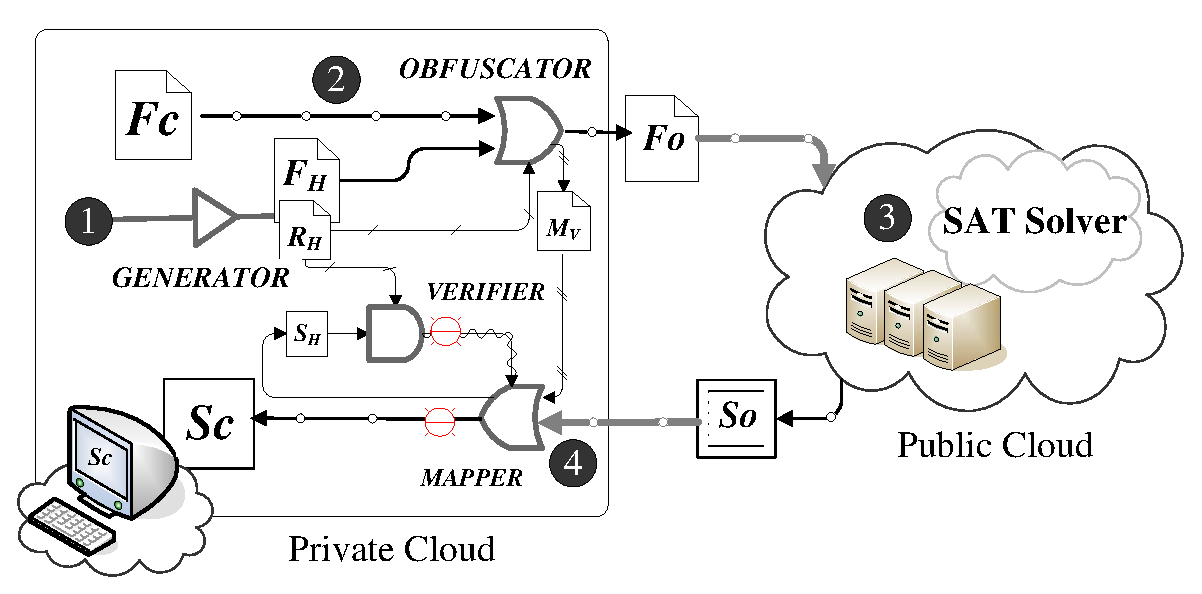
\includegraphics[width=8.2cm]{Visio-cloudsat.eps}}
\caption{Privacy-preserving SAT solving framework based on CNF formula obfuscation.}
\label{fig_cldSAT}
\end{figure}

% \begin{enumerate}
% \item[$\textbf{Step 1,}$]GENERATOR algorithm generates a Husks formula $F_H$ and one of its solution $R_H$.
% \item[$\textbf{Step 2,}$]OBFUSCATOR algorithm obfuscates the Original CNF $F_C$ to obtain a new CNF formula $F_O$.
% \item[$\textbf{Step 3,}$]$F_O$ is solved by SAT Solver deployed in public Cloud, which returns solution $S_O$.
% \item[$\textbf{Step 4,}$]MAPPER and VERIFIER algorithm maps $S_O$ to $S_C$, and check if $F_C$ is satisfied under $S_C$.
% \end{enumerate}

$\textbf{Step 1}$, GENERATOR algorithm generates a Husks formula $F_H$ and one of its solution $R_H$.

$\textbf{Step 2}$, OBFUSCATOR algorithm obfuscates the Original CNF $F_C$ to obtain a new CNF formula $F_O$.

$\textbf{Step 3}$, $F_O$ is solved by SAT Solver deployed in public Cloud, which returns solution $S_O$.

$\textbf{Step 4}$, MAPPER and VERIFIER algorithm maps $S_O$ to $S_C$, and check if $F_C$ is satisfied under $S_C$.

% % $\mathbf{Step 1}$, GENERATOR algorithm generates a Husks formula $F_H$ and one of its solution $R_H$.
% 
% $\mathbf{Step 2}$, OBFUSCATOR algorithm obfuscates the Original CNF $F_C$ to obtain a new CNF formula $F_O$.
% 
% $\mathbf{Step 3}$, $F_O$ is solved by SAT Solver deployed in Cloud, which returns solution $S_O$.
% 
% $\mathbf{Step 4}$, MAPPER and VERIFIER algorithm maps $S_O$ to $S_C$,the sulution  of $F_C$, and check if $F_C$ is satisfied under $S_C$.

The \textbf{Step 3} run in public Cloud, while other steps run in trusted private Cloud.

The GENERATOR, OBFUSCATOR, MAPPER and VERIFIER algorithms will be described in Subsection \ref{genhusk}, \ref{obfuscating}
and \ref{mappping} respectively.

\subsection{Husks formula Generation}\label{genhusk}

There are several methods to generate satisfiable CNF formula\cite{microgenSAT,genSAT}.
In this paper, Husks formula (in Definition \ref{Husks-formula-definition}) is constructed based on prime factorization method,
as described in literature\cite{genSAT}.

GENERATOR algorithm to generate Husks formula is shown in Algorithm \ref{algo2_gen}.
%\subsubsection{Generating Husks formula with unique solution}
%Husks formula is a special satisfied CNF formula,which has unique solution.
%\textbf{First},
%given a prime $p$ represented by a binary vector $p = <p_1,p_2,\dots,p_n>$,
%we assigning its square $p^2$ to the output of a multiplier $M$,with constraint $I_1\ne 1$ and  $I_2\ne 1$.
%while $I_1$ and $I_2$ is inputs of  $M$.
%\textbf{Second},
%We convert the multiplier $M$ into CNF formula $Tseitin(M)$.
%
%To satisfy $Tseitin(M)$,
%the two inputs of $M$ must all be $p = <p_1,p_2,\dots,p_n>$,
%which makes the $p$ the unique solution of $Tseitin(M)$.
%
%\subsubsection{Husk CNF formula with unique cluster solution}
%\textbf{A CNF formula with a unique cluster shaped solution}
%\textbf{A CNF formula with only two solutions}

\textbf{First}, 
given two primes $p_A \neq p_B$ (at line \ref{primenumber}),
% represented by a binary vector $p_A = <a_1,a_2,\dots,a_n>$, $p_B = <b_1,b_2,\dots,b_n>$,
we assign $p_A \cdot p_B$ to the output of a multiplier $M$ with constraint $I_1\ne 1$ and  $I_2\ne 1$ (at line \ref{multiplePrime}).
$I_1$ and $I_2$ are inputs of $M$.

\textbf{Second}, 
we convert the multiplier $M$ into CNF formula $Tseitin(M)$ (at line \ref{TseitinPHI}).

To satisfy $Tseitin(M)$, the two inputs of $M$ must be $\{I_1=p_A,I_2=p_B\}$ or $\{I_1=p_B,I_2=p_A\}$, 
which makes the $p_A|p_B$ or $p_B|p_A$ the two solutions of $Tseitin(M)$.
We take one of them as $R_H$.
% 
% \begin{procedure}
% \item[input]  NULL
% \item[output] Husks CNF $F_H$ and Husks result $R_H$
% \Begin{
% Generating prime numbers $p_A$ and $p_B$  \; \label{primenumber}
% $\Phi= M(I_1 \neq 1, I_2\neq 1, O=p_A*p_B)$ \;\label{multiplePrime}
% $F_H=Tseitin(\Phi)$ \;\label{TseitinPHI}
% $R_H=p_A\mid p_B$ \;
% }
% \caption{GENERATOR}
% \label{algo2_genSAT}
% \end{procedure}

\begin{algorithm}[b]
% \SetAlgoLined
% \SetAlgoNoLine
\KwData{NULL}
\KwResult{Husks CNF $F_H$ and Husks result $R_H$}
\Begin{
Generating prime numbers $p_A$ and $p_B$  \; \label{primenumber}
$\Phi= M(I_1 \neq 1, I_2\neq 1, O=p_A*p_B)$ \;\label{multiplePrime}
$F_H=Tseitin(\Phi)$ \;\label{TseitinPHI}
$R_H=p_A\mid p_B$ \;
}
\caption{GENERATOR}
\label{algo2_gen}
\end{algorithm}

Singular Husk formula with unique solution (in Definition \ref{Singular-Husk-formula-definition}) can also be constructed by similar method described in Algorithm \ref{algo2_gen},
by constraining $p_A\equiv p_B$. 

\subsection{Circuit Structure aware obfuscation}\label{obfuscating}
\subsubsection{Circuit structure in CNF formula}\label{CNF structure}
%\textbf{Circuit structure in CNF formula}\label{CNF structure}
Since we want to protect circuit structure in CNF formula, 
let's first study how the circuit can be recovered from CNF formula.
Literatures\cite{csRoy,csFu} have proposed algorithms to recover circuit structure from CNF formula in details.
Before discussing them, some concepts should be introduced first.

\begin{definition}[CNF signature]
CNF signature of gate $g$ is its Tseitin encoding $Tseitin(g)$.
Each clause in CNF signature is called characteristic clause.
A characteristic clause containing all variables in CNF signature is a \textbf{key clause}.
Variable corresponding to output of a gate is called \textbf{output variable}.
\end{definition}

For AND2 in Equation (\ref{eqn_andinv}), 
$\neg e\vee c$ is a characteristic clause.
Clause $e\vee \neg c\vee\neg d$ is a key clause.
$e$ is an output variable.

As metioned in \cite{csRoy}, 
gates with the same characteristic functions will be encoded into the same CNF signature.

% Some such algorithms\cite{csRoy,csFu} are based on concept of directed hyper-graph.
% 
% \begin{definition}
% [Hypergraph and Directed Hypergraph of CNF]
% A Hypergraph $G=(V,E)$ of a CNF formula $\Sigma$ is
% \begin{enumerate}
%  \item[-] each vertex of $V$ corresponds to a clause of $\Sigma$;
%  \item[-] each edge $(c_1,c_2)\in E$ corresponds to two clauses $c_1$ and $c_2$ containing the same variable or its negation;
%  \item[-] each edge is labeled by the variable;
% \end{enumerate}
% A Directed Hypergraph is a Hypergraph with each endpoint of edge labeled
% by plus when clause contains positive variable, 
% or minus when clause contains negative variable.
% \end{definition}
With these definitions, 
Roy et al. \cite{csRoy}
first converts the CNF to an Hypergraph $G$, 
and then matches the CNF signatures of all types of gates in $G$ to recover gates by subgraph isomorphism, 
finally creates a maximal independent set instance to represent the recovered circuit.

Fu et al.\cite{csFu} presents another algorithm that
first detects all possible gates with key clause and CNF signature based pattern matching, 
and then constructs a maximum acyclic combinational circuit by selecting a maximum subset of matched gate.

Potential attackers can exploit these knowledge to recover the circuit structure.
Thus, CNF signature and key clause are important information that should be protected.

\subsubsection{Input and output privacy-preserving scheme}
To prevent information carried by CNF formula and its solution from leakage, a privacy-preserving scheme is proposed,
the scheme is based on the following facts and anticipations:
\\$\textbf{Fact 1:}$ Changing CNF signature and key clause in CNF formula will make circuit recovering
based on pattern matching or subgraph isomorphism impossible.
\\$\textbf{Fact 2:}$ Solution space should not be under-approximated after obfuscation, otherwise the result will be misleading even for real user.
\\$\textbf{Anticipation 1:}$ According to Fact 2, solution space have to be over-approximated  after obfuscation, so as to mislead hoarding participants in public Cloud.
\\$\textbf{Anticipation 2:}$ The solution of obfuscated CNF formula should be easily mapped back to the original formula.
% \begin{enumerate}
% \item[]$\textbf{Fact 1,}$ 
%  Changing CNF signature and key clause in CNF formula will make circuit recovering
%  based on pattern matching or subgraph isomorphism impossible.
% \item[]$\textbf{Fact 2,}$ 
%  Solution space should not be under-approximated after obfuscation, otherwise the result will be misleading even for real user.
% \item[]$\textbf{Anticipation 1,}$
%  According to fact 2, solution space have to be over-approximated  after obfuscation, so as to mislead hoarding participants in public Cloud.
% \item[]$\textbf{Anticipation 2,}$
%  The solution of obfuscated CNF formula should be easily mapped back to the original formula.
% \end{enumerate}

The proposed scheme, denoted as OBFUSCATOR, generates a new CNF formula $F_O$, 
by embedding Husks formula $F_H$ into the original formula $F_C$, 
with Circuit Structure Aware(CSA) strategy and Solution Space Hold(SSH) rules .
By CSA strategy, 
the scheme changes the clause set and literal set in clauses of $F_C$, 
to prevent its structure from being recovered.
By SSH rules, 
the solution space is over-approximated after obfuscation, 
so as to prevent its accurate solutions from being known even by SAT solver in public Cloud.
% We will describe them below in \ref{embeded rules}) and \ref{embeded strategy}) respectively. 
We will describe them below in Subsection \textit{\ref{embeded rules}}) and \textit{\ref{embeded strategy}}) respectively. 

\subsubsection{Solution Space Hold rules}\label{embeded rules}
% In order to blend a CNF formula $F_C$ with $F_H$ seamlessly, 
% OBFUSCATOR will insert variables of $F_H$ into clauses of $F_C$, 
% and generate new clauses with variables in $F_C$ and $F_H$.
% When inserting variables or generating new clause, 
% OBFUSCATOR will obey the Solution Space Hold(SSH) rules, 
% so as to make the solution space over-approximated but under control.
Let's consider an interesting problem:
We outsource CNF formula generated from SAT problem, 
and wish SAT solver deployed in Cloud to give solutions to the SAT problem,
without knowing exactly what the SAT problem is and what the exactly solution is.

A simple approach is to blend CNF formula of real SAT problem with that of another satifiable SAT problem,
and outsource the blended CNF formula.
Unfortunately, partition based technique \cite{Partition} can easily separate the two undependent formulas. 

Let's consider an incremental approach:
An arbitrary formula $F_C$,
and a satisfiable formula $F_H$ with \textsl{${\textbf{R}}_{\textbf{H}}$} as one of its solutions,
and there is no common variable between $F_C$ and $F_H$, viz.$V_{F_C}$ $\cap$ $V_{F_H}$ =$\phi$.
We blend $F_C$ with $F_H$ seamlessly, so as to hide $F_C$.
At the same time, we keep all solutions of $F_C$ still in the new formula. 

To blend $F_C$ and $F_H$ seamlessly,
an intuitive approach is to insert variables of $F_H$ into clauses of $F_C$, 
and generate new clauses with variables in $F_C$ and $F_H$. According to property of CNF, for any CNF formula $F_C$, 
inserting new variables into its clauses may expand its solution space; 
On the contrary,
adding new clauses which consist variables in $F_C$,
may narrow down its solution space. 
How can we ensure all the solutions of $F_C$ still in new formula?
Before giving answer to this problem,
following concepts should be clarified.

\begin{definition}[$ Solution~S_C \subseteq Solution~S_O$]~
CNF formula $F_C$ and $F_O$ have $n_{F_C}$ common variables $x_1,...,x_{n_{F_C}}$ and
$|V_{F_C}|\equiv n_{F_C}$, $|V_{F_O}|\equiv n_{F_O}$, $ n_{F_O}\geqslant n_{F_C} > 0$.
$S_C$ and $S_O$ are solutions of $F_C$ and $F_O$ respectively, 
and assignments to $n_{F_C}$ common variables are same in $S_C$ and $S_O$, viz.
~~$S_C=\{x_1=B_1,...,x_{n_{F_C}}=B_{n_{F_C}} | B_i \in \{T,F\},~1\leqslant i\leqslant n_{F_C} \}$,\\
~~$S_O=\{x_1=B_1,...,x_{n_{F_C}}=B_{n_{F_C}},...,x_{n_{F_O}}=B_{n_{F_O}}|B_i\in \{T,F\},~ 1\leqslant i\leqslant n_{F_O} \}$.
Then Solution $S_C$ is subset of Solution $S_O$,
denoted as $S_C \subseteq S_O$.
\end{definition}

\begin{definition}[Solution Space Equation(SSE)]\label{SSEdefinition}~
CNF formula $F_C$ has $n$ solutions $\{S_{C_1},...,S_{C_n}\}$;
By obfuscation,
$F_C$ has been transformed into $F_O$,
which also has $n$ solutions $\{S_{O_1},...,S_{O_n}\}$,
and for $i \in [1,n]$, $S_{C_i} \subseteq S_{O_i}$.
Then, we say $F_O$ is solution space equated with $F_C$, 
denoted as  $F_C \equiv_{_{SSE}} F_O$.
\end{definition}

\begin{definition}[Solution Space Over-approximation(SSO)]\label{SSOdefinition}~
CNF formula $F_C$ has $n$ solutions $\{S_{C_1},...,S_{C_n}\}$;
By obfuscation,
$F_C$ has been transformed into $F_O$,
which has $m$ solution, $\{S_{O_1},...,S_{O_n},...,S_{O_m}\}$,
$m \geqslant n$,
while for $i \in [1,n]$, $S_{C_i} \subseteq S_{O_i}$.
Then, we say $F_O$ is solution space over-approximated as $F_C$, 
 denoted as $F_C \vdash_{_{SSO}} F_O$.
\end{definition}

In order to keep all solutions of $F_C$ in new formula,
we proposed Solution Space Hold(SSH) rules to obfuscate $F_C$ with $F_H$ and one of its solutions $R_H$,
so as to make the solution space over-approximated after obfuscation.

\textbf{Solution Space Hold Rules (SSH Rules): }
\begin{enumerate}
\item \textbf{Rule 1}:
For any clause $c\in F_{C}$, 
take one variable from $R_H$, 
and insert it into $c$ according to the following rule:
If assignment of variable is $T$ in $R_H$, insert its negative literal;
If assignment of variable is $F$ in $R_H$, insert its positive literal.
Then clause $c$ is replaced with the resulted clause.
\item \textbf{Rule 2}:
%generating new clauses with literals from $R_H$ and output variables in $F_C$ according to the following rule:
Generating new clauses with literals from $R_H$ and variables in $F_C$ according to the following rule:
If assignment of variable is $T$ in $R_H$, insert positive literal into clause;
If assignment of variable is $F$ in $R_H$, insert negative literal into clause.
%Literal of output variable is extracted directly from the key clause and inverted.
\end{enumerate}

\begin{definition}[${\textbf{Obf(}}F_C,F_H,R_H\textbf{)}$]\label{OBFUSCATORSSH}
For arbitrary formula $F_C$, and satisfiable formula $F_H$ with $R_H$ as one of its assignments, 
$Obf(F_C,F_H,R_H)$ is the result of applying SSH Rules when blending $F_C$ with $F_H$.
If $F_H$ is a Singular Husk formula and $R_H$ is its unique solution, $Obf(F_C,F_H,R_H)$ is called ${\textbf{SSE obfuscation}}$.
If $F_H$ is Husks formula and $R_H$ is one of its solutions, $Obf(F_C,F_H,R_H)$ is called ${\textbf{SSO obfuscation}}$.
\end{definition}

% \begin{definition}[${\textbf{Obf(}}F_C,F_H,R_H\textbf{)}$]\label{OBFUSCATORSSH}
% For arbitrary formula $F_C$, and satisfiable formula $F_H$ with $R_H$ as one of its solutions, 
% $Obf(F_C,F_H,R_H)$ is the result of applying SSH Rules when blending $F_C$ with $F_H$.
% If $F_H$ is a Singular Husk formula, $Obf(F_C,F_H,R_H)$ is called ${\textbf{SSE obfuscation}}$.
% If $F_H$ is Husks formula, $Obf(F_C,F_H,R_H)$ is called ${\textbf{SSO obfuscation}}$.
% \end{definition}

For SSH based obfuscation, we have following theorems.

\begin{theorem}[SSE Obfuscation]\label{SSEtheorem}

For arbitrary CNF formula $F_C$, and Singular Husk formula $F_{_SH}$, 
if $V_{F_C} \cap V_{F_{_SH}} \equiv \phi$, and
$R_{_SH}$ is the unique solution of $F_{_SH}$,
\textbf{then} $Obf(F_C,F_{_SH},R_{_SH}) \equiv F_C\wedge F_{_SH}$.
\end{theorem}

\begin{theorem}[SSO Obfuscation]\label{SSOtheorem}
For arbitrary CNF formula $F_C$, Husks formula $F_H$, if 
$V_{F_C} \cap V_{F_H} \equiv \phi$, and
$R_H$ is one of solutions of $F_H$.  
\textbf{then} $F_C \vdash_{_{SSO}} Obf(F_C,F_H,R_H)$.
% \textbf{then} $F_C\wedge F_H \vdash F_O$.
\end{theorem}

According to Theorem \ref{SSEtheorem} and Definition \ref{SSEdefinition}, we have:
% inference \ref{SSEinference}.
\begin{inference}\label{SSEinference}
For arbitrary CNF formula $F_C$, Singular Husk formula $F_{_SH}$, if
$V_{F_C}\cap V_{F_{_SH}}\equiv \phi$, and
$R_{_SH}$ is the unique solution of $F_{_SH}$,
\textbf{then} $Obf(F_C,F_{_SH},R_{_SH}) \equiv_{_{SSE}} F_C$.
\end{inference}

Theorem \ref{SSEtheorem} and \ref{SSOtheorem} will be proved in Subsection \ref{correctness}.

An obfuscated CNF formula $F_O=Obf(F_C,F_H,R_H)$ generated by SSO obfuscation 
consists of all the variables of $F_C$ and $F_H$.

If variables from $F_H$ are assigned with $R_H$, then we have:

$F_O(R_H/V_{F_O})
=Obf(F_C,F_H(R_H/V_{F_H}),R_H)$ 

Accdording to Lemma \ref{HE} in Subsection \ref{correctness}, 
$F_H(R_H/V_{F_H})$ can be expressed as a Singular Husk formula with unique solution $R_H$.
According to Inference \ref{SSEinference}, for CNF formulas $F_C$  and its obfuscated formula $F_O$, we have:
\begin{enumerate}
 \item $F_C$  is unsatisfiable iff $F_O$ is unsatisfiable.
 And the unsatisfiable core of $F_C$  can be obtained from unsatisfiable core of $F_O$ by deleting literals in $F_H$.
 \item $F_C$  is satisfiable iff $F_O$ is satisfiable.
 And the solution of $F_C$  can be obtained by projecting solution of $F_O$ into variables set of $F_C$ .
\end{enumerate}

As a result, each solution of $F_O$ can be partitioned into solutions of $F_C$ and $F_H$. So
the solution of $F_C$ can be extracted from that of $F_O$ by projection on variables set of $F_C$.

If variables from $F_H$ are assigned with other solution except $R_H$, that is $(S_H\neq R_H)$, then we have:

$F_O(S_H/V_{F_O})
=Obf(F_C,F_H(S_H/V_{F_H}),R_H)$.

Since $R_H$ is not solution of $F_H(S_H/V_{F_H})$, obfuscation may expand solution space of $F_C$, that is:
If $F_O$ is satisfied, solution acquired by projection on variables set of $F_C$ may be false solution.
We can rule out this situation by confining $F_H$ being assigned with $R_H$ when recovering solution.

In conclusion, the solution space of $F_O$ is overapproximation of $F_C$.
As a result,
$F_O$ can be solved with the same SAT solver as $F_C$, 
but solution of $F_C$ can not be recovered from that of $F_O$ without knowing $R_H$.

\begin{algorithm}[t]
% \SetLine
\KwData{The original CNF $F_C$, Husks CNF $F_H$, Husks result $R_H$}
\KwResult{The obfuscated CNF $F_O$, variable mapping $M$}
\Begin{
$mark(F_C)$\;\label{mark}
\ForEach{$c\in F_C$}{
\If{$c \in$  Key Clause Set } {\label{keyclause}
    lit =get literal $ \in R_H$\;
    $c=c \cup \neg lit$\;\label{rule1}
    $nc=generate\_new\_clause(c,lit)$\;\label{gennewclause}
    $F_C=F_C \cup nc$\;\label{blendclause1}
 }
}
\ForEach{$ c \in F_C $} {
$averagelen=\frac{\sigma _{c'\in F_C}|c'|}{|F_C|}$ \;
\While{$|c| < averagelen$}{
$lit=$get literal $\in R_H$ \;
\While{$\neg lit \in c$} {
lit=get literal $ \in R_H $ \;
}
$c=c \cup \neg lit$\;\label{rule1-2}
}
$M$ =remap all variable in $F_C\cup F_H$ \;\label{MV}
$F_O$ =reorder all clause in $F_C\cup F_H$ \; \label{blendclause2}
}
}
\caption{OBFUSCATOR}
\label{algo_obs}
\end{algorithm}

\begin{algorithm}[t]
% \SetAlgoNoLine
$\mathbf{mark}$\;
\KwData{CNF formula $S$}
\KwResult{marked $S$ }
\Begin{
\ForEach{$(C \in S) ~\&~ (|C|\equiv 3)$}{
\ForEach{$l \in C$ }{
\ForEach{$(C_1 \in S) ~\&~ (\neg l\in C_1)~ \&~ (|C_1|\equiv 2)$ }{
\ForEach{$l_1 \in C_1$ }{
\uIf{$(\neg l_1 \in C)~\&~(l_1\ne l)$} {
$match++$ \;
}
}
}
}
}
\If{$match\equiv 2$} {
mark $l$ as output literal \;
mark $C$ as Key Clause\;
}
}
$\mathbf{generate\_new\_clause}$\;
\KwData{key clause $C$ in AND2, Husk literal $lit$}
\KwResult{new clause $C_1$}
\Begin{
$olit$=Getting output literal from $C$ \;
$C_1= lit \cup \neg olit$ \;\label{rule2}
}
\caption{$\mathbf{mark}$ and $\mathbf{generate\_new\_clause}$}
\label{algo_mark}
\end{algorithm}


\subsubsection{Circuit Structure Aware strategy}\label{embeded strategy}
Through SSH, OBFUSCATOR can insert new literals into clauses and generate new clauses, 
while ensuring the solution space under control.
But which clause should be inserted with literal and what forms of new clause should be generated remain a question.

Since gates are basic blocks to construct circuit, 
and CNF signature and key clause are clues to detect circuit structure, 
as mentioned in Subsection \textit{\ref{CNF structure})}.
We try to change the CNF signature and key clause of gate by adding literals and clauses.
Furthermore, in order to mislead adversary, 
literals and clauses added may construct new legal CNF signature with clauses in original CNF signature, 
so as to hide original circuit structure seamlessly.

For example, Figure\ref{fig_AND2}a) is CNF signature of AND2 gate $a$.
By inserting A into key clause $c_1$ and generating clause $c_4$ with $A$ and $a$, 
we transform gate $a$ from AND2 into AND3, with a new input variable $A$, 
which is distinguishable with $b$ and $c$, the input variables of AND2.
The clauses for OR, NAND, and NOR gates, 
which are quite similar to that of AND gates,
can also be transformed in this way. 

\begin{figure}
\footnotesize\centering
\centerline{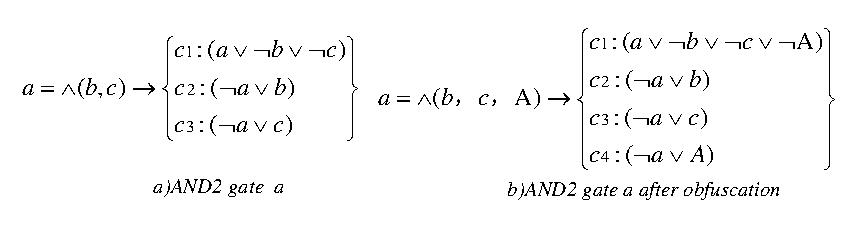
\includegraphics[width=9.2cm]{AND2.eps}}
\caption{Obfuscating AND2 into AND3.}\centering
\label{fig_AND2}
\end{figure}

\subsubsection{All in One}\textsl{OBFUSCATOR algorithm}

The proposed OBUFSCATOR algorithm obfuscates CNF formula $F_C$ with SSH rules and CSA strategies, 
so as to prevent structure of $F_C$ and its accurate solution from being known by adversary.

To achieve these goals, OBFUSCATOR detect gates in CNF formula, 
then transform them into gates with different CNF signature.
Detailed implementation of OBFUSCATOR is in Algorithm \ref{algo_obs}, which use $mark$ $($line \ref{mark}$)$ to detect key clauses and output variables  in CNF formula, 
and use $generate\_new\_clause$ $($line \ref{gennewclause}$)$ to generate new clause.
As all circuits can be represented by a combination of AND2 and INV, 
and the $mark$ algorithm for INV is trivial, 
so we only present the implementation of $mark$ for AND2 in Algorithm \ref{algo_mark}.
Similarly, we also present only the implementation of $\mathbf{generate\_new\_clause}$ for AND2 in Algorithm \ref{algo_mark}.
These two algorithms can transform a CNF signature of AND2 to that of AND3.


SSH and CSA based obfuscation procedure implemented in Algorithm \ref{algo_obs} and \ref{algo_mark} is described below.
% \textbf{SSO obfuscation with SSH rule and CSA strategy}
\begin{Procedure}[${Obf_{SSH\_CSA}}$]\label{obsprocedure}~
\begin{enumerate}
\item Input:
Formula $F_C$, Husks formula $F_H$, solution $R_H$.
\item Output:
Formula $F_O$.
\end{enumerate}
According to Algorithm \ref{algo_obs}, 
$F_C$ consists of \textbf{key clause}(line \ref{keyclause}) and \textbf{non-key clause}, 
corresponding clause sets denoted as \textbf{$F_{Ck}$} and \textbf{$F_{Cn}$}.

% $~~~~R_H$ is one sultion of $F_H$.
\textbf{Step 1}: 
For key clause $c\in F_{Ck}$, 
take one literal lit from $R_H$, 
and insert $\neg lit$ into $c$ (at line \ref{rule1}, \ref{rule1-2} in Algorithm \ref{algo_obs})  according to  SSH rule 1.
% if variable is $T$ in $R_H$, insert its negative literal;
% if variable is $F$ in $R_H$, insert its positive literal.
The resulting clause set is denoted as $S_3$ .

\textbf{Step 2}: 
Generating new clauses  (line \ref{gennewclause} in Algorithm \ref{algo_obs}) with literal lit from $R_H$ and output variable of $c$ in $F_C$ according to SSH rule 2 (line \ref{rule2} in Algorithm \ref{algo_mark}).
% %generating new clauses with literals from $R_H$ and variables in $F_C$ according to the SSH rule 2:
% if variable is $T$ in $R_H$, insert positive literal into clause;
% if variable is $F$ in $R_H$, insert negative literal into clause;
% %Literal of output variable is extracted directly from the key clause and inverted.
New clauses set generated in this way is denoted as $S_4$.

\textbf{Step 3}: 
Combining and randomly reordering $S_3$, $S_4$, $F_H$, and $F_{Cn}$, to produce $F_O$ (line \ref{rule1}, \ref{rule1-2}, \ref{blendclause1} \ref{blendclause2} in Algorithm \ref{algo_obs}).

\textit{\textbf{end Procedure}}.
\end{Procedure}

\subsection{Solution recovery}\label{mappping}
After SAT Solving finished in public Cloud, $S_O$, 
the solution of $F_O$, will be returned to the private Cloud.
In accordance with OBFUSCATOR, 
MAPPER and VERIFIER are used to filter solution of $F_C$ out from  $S_O$.
MAPPER and VERIFIER are implemented in Algorithm \ref{algo_map}.

According to Theorem \ref{SSOtheorem},
If result is UNSAT, then the original CNF formula is UNSAT (line \ref{sUNSAT}).
If result is SAT, MAPPER (line \ref{var}-\ref{mapper}) projects solution into variables of $F_C$ and $F_H$, 
to get $S_C$ and $S_H$, which are the candidate solution of $F_C$ and $F_H$ respectively.
VERIFIER (line \ref{verifer1}-\ref{verifer2}) checks if $S_H$ is equal to $R_H$, 
if yes, $S_C$ is real solution of  $F_C$.
Otherwise, $S_C$ may be false solution,
hence, it is necessary to ask for a new solution from SAT Solver(at line \ref{Warning}).

The solution projection is done according to the variable mapping table $M$, 
generated by OBFUSCATOR(at Line \ref{MV} in Algorithm \ref{algo_obs}).
$M[var].variable$ (at Line \ref{var}) represents the original variables name of var, 
and $M[var].formula$ (at Line \ref{formula}) may be $F_C$ or $F_H$, which the var belongs to.

\begin{algorithm}[t]
% \SetAlgoNoLine
\KwData{Obfuscated result $S_O$, variable mapping table $M$, Husk result $R_H$}
\KwResult{Result $S_C$}
\Begin{
\ if {$S_O$ is UNSAT} {\label{sUNSAT}
    return UNSAT \;
 }
\ForEach{$lit \in S_O$} {
$var=abs(lit)$\;
$rvar=M[var].variable $\;\label{var}
\eIf{$M[var].formula ~is~ F_C$} { \label{formula}
$S_C[rvar]=lit>0?rvar:\neg rvar$ \; \label{mapper}
}
{
$Hlit=lit>0?rvar:\neg rvar$\;\label{verifer1}
\uIf{$R_H[rvar]\ne Hlit$}{ 
    alert("Get another Solution from SAT Solver")\; \label{Warning}
    break;
}
}\label{verifer2}
}
 printf(" SAT  solution is $S_C$ ");
}
\caption{MAPPER and VERIFIER}
\label{algo_map}
\end{algorithm}
\section{Correctness, Effectiveness and Complexity}
\subsection{Correctness}\label{correctness}
According to Theorems \ref{SSEtheorem} and \ref{SSOtheorem}, under SSH rules, 
original CNF formula can be blended with Husks formula seamless, without narrowing down the solution space.
In this section, we prove these theorems.
First of all, let's introduce some lemmas.


% \begin{lemma}[Husks Equation]\label{HE}
% 
% For Husks formula ${F_H}$ with one of its solutions $S_H$,
% and $|V_{F_H}|= n$, and \\
% $S_H$=$\{(y_i=B_i,y_j=B_j)|B_i\equiv T, B_j\equiv F, ~~1\leqslant i, j\leqslant n \}$.\\
% let $F_{_SH}=F_H\wedge (\bigwedge_{1\leqslant i\leqslant n}^{B_i\equiv T}y_i)\wedge(\bigwedge_{1\leqslant j\leqslant n}^{B_j\equiv F}\neg y_j)$\\
% then $F_{_SH} \vdash F_H $.
% \end{lemma}
% 
% \begin{proof}
% 
% Since $F_{_SH}\equiv T$ and \\  
% $F_{_SH}=(\bigwedge_{1\leqslant i\leqslant n}^{B_i\equiv T}y_i)\wedge(\bigwedge_{1\leqslant j\leqslant n}^{B_j\equiv F}\neg y_j$,\\ 
% then must have \\
% $\{(y_i=T,y_j=F)|B_i\equiv T, B_j\equiv F, ~~1\leqslant i, j\leqslant n \}$,\\
% let $S_H$=$\{(y_i=T,y_j=F)|B_i\equiv T, B_j\equiv F, ~~1\leqslant i, j\leqslant n \}$,\\
% let $B_i$ substitutes $T$, $B_j$ substitutes $F$,\\
% then  $S_H$=$\{(y_i=B_i,y_j=B_j)|B_i\equiv T, B_j\equiv F, ~~1\leqslant i, j\leqslant n\}$\\
% $S_H$ is one solution of $F_H$, then  $F_H(S_H/V_{F_H}) $ is true.\\
% then $F_{_SH} \vdash F_H $.
% 
% \textit{end proof.}
% \end{proof}

%%%%%%%%%%%%%%%%%%%%%%%%%%%%%%%%%%%%%%%%%%%%%%%%%%%%%%%%%%%%%%%%%%%%%%%%%%%%%%%%%%%%%%55
\begin{lemma}[Husks Equation(HE)]\label{HE}

For Husks formula ${F_H}$ and $|V_{F_H}|= n$,
with its all $m$ solutions $\{S_{H_l}|1\leqslant l\leqslant m\}$,
and $S_{H_l}=\{y_k=B_{l_k}|B_{l_k} \in \{T,F\}, 1\leqslant k\leqslant n\}$.

For each $S_{H_l}$, let $F_{slH}=
(\bigwedge_{1\leqslant i\leqslant n}^{B_{l_i}\equiv T}y_{i})\wedge 
(\bigwedge_{1\leqslant j\leqslant n}^{B_{l_j}\equiv F}\neg y_{j})$,

and $F_{_SH}=\bigvee_{1\leqslant l\leqslant m}F_{slH}$,

\textbf{then}  $F_{_SH} \equiv F_H $.
\end{lemma}

\begin{proof} \\
1) Since $F_{_SH} \equiv T$ then there must exist
% $F_{slH}\equiv T$, for
\begin{equation}
F_{slH}=
(\bigwedge_{1\leqslant i\leqslant n}^{B_{l_i}\equiv T}y_{i})\wedge 
(\bigwedge_{1\leqslant j\leqslant n}^{B_{l_j}\equiv F}\neg y_{j}) \equiv T
\end{equation}
Then we have:
\begin{equation}
S_{H_l}=\{y_{i}=T,y_{j}=F|B_{l_i}\equiv T, B_{l_j}\equiv F, 1\leqslant i, j\leqslant n \} 
\end{equation}
Let $B_i$, $B_j$ substitutes $T$ in $y_{i}=T$ and $F$ in $y_{j}=F$ respectively, then we have
\begin{equation}
S_{H_l}=\{(y_i=B_{l_i},y_j=B_{l_j})|B_{l_i}\equiv T, B_{l_j}\equiv F, 1\leqslant i, j\leqslant n\} 
\end{equation}
Since $S_{H_l}$ is one solution of $F_H$, then  $F_H(S_H/V_{F_H}) $ is true. thus we have:
\begin{equation}\label{left}
 F_{_SH} \vdash F_H
\end{equation}
2) Since $F_H\equiv T$, then there exists a solution of $F_H$,
shown in Equation (\ref{solution_hl}), that make $F_H(S_{H_1}/V_{F_H})$ true.
\begin{equation}\label{solution_hl}
S_{H_1}=\{y_k=B_{1_k}|B_{1_k} \in \{T,F\}, 1\leqslant k\leqslant n\}.
\end{equation}
Construct $F_{s1H}$ according to (\ref{solution_hl}), and we have Equation (\ref{SH}):
\begin{equation}\label{s1H}
F_{s1H}=
(\bigwedge_{1\leqslant i\leqslant n}^{B_{1_i}\equiv T}y_{i})\wedge 
(\bigwedge_{1\leqslant j\leqslant n}^{B_{1_j}\equiv F}\neg y_{j})
\end{equation}
\begin{equation}\label{SH}
F_{_SH} =F_ {s1H} \vee (\bigvee_{2\leqslant l\leqslant m}F_{slH}). \\
\end{equation}
Since $F_{s1H} \equiv T$, with Equation (\ref{s1H}) and (\ref{SH}), we have: 
\begin{equation}
F_{_SH}  \equiv T 
\end{equation}
\begin{equation}\label{right}
F_H \vdash F_{_SH}
\end{equation}
According to Equation (\ref{left}) and (\ref{right}), we have:
\begin{equation}
 F_{_SH} \equiv F_H 
\end{equation}
%\textit{end proof.}
\end{proof}

\begin{lemma}[Singular Husk Equation(SHE)]\label{SHE}

For singular Husk formula ${F_H}$ with $|V_{F_H}|= n$,
and unique solutions $S_H$=$\{(y_i=B_i,y_j=B_j)|B_i\equiv T, B_j\equiv F, 1\leqslant i, j\leqslant n \}$.

let $F_{_SH}=F_H\wedge (\bigwedge_{1\leqslant i\leqslant n}^{B_i\equiv T}y_i)\wedge(\bigwedge_{1\leqslant j\leqslant n}^{B_j\equiv F}\neg y_j)$

\textbf{then} $F_H \equiv F_{_SH}$.
\end{lemma}
\begin{proof}
\textsl{Abbr}. Similar to Lemma \ref{HE}.
\end{proof}
%%%%%%%%%%%%%%%%%%%%%%%%%%%%%%%%%%%%%%%%%%%%

% \begin{lemma}[Singular Husk Equation(SHE)]\label{SHE}
% 
% For singular Husk formula ${F_H}$ with $|V_{F_H}|= n$,
% and unique solutions $S_H$,
% with $S_H$=$\{(y_i=B_i,y_j=B_j)|B_i\equiv T, B_j\equiv F, 1\leqslant i, j\leqslant n \}$.
% let $F_{_SH}=F_H\wedge (\bigwedge_{1\leqslant i\leqslant n}^{B_i\equiv T}y_i)\wedge(\bigwedge_{1\leqslant j\leqslant n}^{B_j\equiv F}\neg y_j)$
% 
% \textbf{then} $F_H \equiv F_{_SH}$.
% \end{lemma}
% 
% \begin{proof}
% there are two cases,\\
% % \begin{enumerate}  
% % \item \label{sigularassgn1} $F_H \vdash F_{_SH}$ proof:
% 1)$F_H \vdash F_{_SH}$
% 
% $F_H\equiv T$, $S_H$ is unique solution, and\\  
% $S_H$=$\{(y_i=B_i,y_j=B_j)|B_i\equiv T, B_j\equiv F, 1\leqslant i, j\leqslant n \}$.\\
% let $F_{_{lS}H}=(\bigwedge_{1\leqslant i\leqslant n}^{B_i\equiv T}y_i)\wedge(\bigwedge_{1\leqslant j\leqslant n}^{B_j\equiv F}\neg y_j)$,
% then $F_{_{lS}H} \equiv T $.\\
% let $F_{_SH}=F_H\wedge F_{_{lS}H}$, then $F_{_SH}\equiv T$.
% So $F_H \vdash F_{_SH}$\\
% \\
% 2)$F_{_SH}\vdash F_H$: 
% 
% $F_{_SH}\equiv T$,
% and $F_{_SH}=(\bigwedge_{1\leqslant i\leqslant n }^{B_i\equiv T}y_i)\wedge(\bigwedge_{1\leqslant j\leqslant n}^{B_j\equiv F}\neg y_j)$ \\
% then $S_H$=$\{(y_i=T,y_j=F)|B_i\equiv T, B_j\equiv F, 1\leqslant i, j\leqslant n \}$ is unique solution of $F_{_SH}$.\\  
% let $B_i$ substitutes $T$, $B_j$ substitutes $F$,
% then \\ $S_H$=$\{(y_i=B_i,y_j=B_j)|B_i\equiv T, B_j\equiv F, 1\leqslant i, j\leqslant n \}$\\
% Since $S_H$ is solution of $F_H$, then  $F_H(S_H/V_{F_H})\equiv T$.\\
% So $F_H \vdash F_{_SH}$
% \\
% \\
% According to 1) and 2):
% % $F_{_SH} \vdash F_H $ and $F_H \vdash F_{_SH} $,\\
% then $F_H \equiv F_{_SH}$.
% % \end{enumerate}
% 
% %\textit{end proof.}
% \end{proof}

% \begin{lemma}[Husks Equation(HE)]\label{HE}
% 
% For Husks formula ${F_H}$ and $|V_{F_H}|= n$,
% with its all $m$ solutions $\{S_{H_l}|1\leqslant l\leqslant m\}$,and
% $S_{H_l}=\{y_k=B_{l_k}|B_{l_k} \in \{T,F\}, 1\leqslant k\leqslant n\}$.\\
% For each $S_{H_l}$, let $F_{slH}=
% (\bigwedge_{1\leqslant i\leqslant n}^{B_{l_i}\equiv T}y_{i})\wedge 
% (\bigwedge_{1\leqslant j\leqslant n}^{B_{l_j}\equiv F}\neg y_{j})$,\\
% let $F_{_SH}=\bigvee_{1\leqslant l\leqslant m}F_{slH}$,
% \textbf{then}  $F_{_SH} \equiv F_H $.
% \end{lemma}
% 
% \begin{proof} 
% There are two cases,\\
% 1) $F_{_SH} \vdash F_H $:
% 
% Since $F_{_SH} \equiv T$ then there must exist $F_{slH}\equiv T$,\\
%   for $F_{slH}=
% (\bigwedge_{1\leqslant i\leqslant n}^{B_{l_i}\equiv T}y_{i})\wedge 
% (\bigwedge_{1\leqslant j\leqslant n}^{B_{l_j}\equiv F}\neg y_{j})$,\\
% then we have 
% $S_H$=$\{y_{i}=T,y_{j}=F|B_{l_i}\equiv T, B_{l_j}\equiv F, 1\leqslant i, j\leqslant n \}$,\\
% let $B_i$ substitutes $T$ in $y_{i}=T$, $B_j$ substitutes $F$ in $y_{j}=F$,\\
% then we have $S_H$=$\{(y_i=B_{l_i},y_j=B_{l_j})|B_{l_i}\equiv T, B_{l_j}\equiv F, 1\leqslant i, j\leqslant n\}$\\
% $S_H$ is one solution of $F_H$, then  $F_H(S_H/V_{F_H}) $ is true.\\
% So $F_{_SH} \vdash F_H $.
% \\
% \\
% 2) $F_H \vdash F_{_SH} $:
% 
% Since $F_H\equiv T$, 
% then there exists $S_{H_l}$, which is one solution of $F_H$, that make $F_H(S_{H_l}/V_{F_H}) $ true. \\
% for $S_{H_l}=\{y_k=B_{l_k}|B_{l_k} \in \{T,F\},1\leqslant l\leqslant m, 1\leqslant k\leqslant n\}$.\\
% construct $F_{slH}$, then $F_{slH} \equiv T$,
% then $F_{_SH} =\bigvee_{1\leqslant l\leqslant m}F_{slH} \equiv T$.
% So $F_H \vdash F_{_SH} $
% \\
% \\
% According to 1) and 2):
% %  $F_{_SH} \vdash F_H $ and $F_H \vdash F_{_SH} $,\\
%  then $F_{_SH} \equiv F_H $.
%  
% %\textit{end proof.}
% \end{proof}

% $F_H$ and its one solution $R_H$=$\{(y_1=B_1,...,y_n=B_n), B_k \in \{T,F\}, 1\leqslant k\leqslant n\}$.\\
%         and its other all $m-1$ solutions\\
%         $S_{H_l}=\{(y_1=B_{l_1},...,y_n=B_{l_n}), B_{l_k} \in \{ T,F \}, 1\leqslant l\leqslant m-1, 1\leqslant k\leqslant n\}$. 
%         
%         let $F_{_SH}=(\bigwedge_{1\leqslant i\leqslant n}^{B_i\equiv T}y_i)\wedge (\bigwedge_{1\leqslant j\leqslant n}^{B_j\equiv F})$\\
%         let $F_{lH}=\bigvee_{1\leqslant l\leqslant m-1}((\bigwedge_{l_1\leqslant i\leqslant n}^{B_{l_i}\equiv T}y_{l_i})\wedge (\bigwedge_{l_1\leqslant j\leqslant n}^{B_{l_j}\equiv F}))$\\
%         $F_H \equiv F_{_SH} \vee F_{lH}$ 
%                 
According to Lemma \ref{HE} and \ref{SHE},
a singular Husk formula is equivalent to conjunction of all its solution literals,
and a Husks formula is equivalent to disjunction of its solutions clauses, 
while each solution clause is conjunction of literals in the solution.

\begin{lemma}[OR Hold Obfuscation]\label{ORrelation-Holding-Obfuscation}
For formula $F_C$ and $F_{_RH}\vee F_{_SH}$, with $R_H$ is an assignment of $F_{_RH} \vee F_{_SH}$,
then

$Obf(F_C,F_{_RH}\vee F_{_SH},R_H)\equiv Obf(F_C,F_{_RH},R_H) \vee Obf(F_C,F_{_SH},R_H)$
\end{lemma}
\begin{proof}
Assume
\begin{enumerate}
 \item[-]$F_C$=$F_{Ck} \wedge F_{Cn}$,  $F_{Ck}$= $\bigwedge_{1}^{m}(a_i\vee X_i$).  
 \item[-]$F_H$=$F_{_RH}\vee F_{_SH}$
 \item[-]$R_H$=$\{y_j=B_j| B_j \in \{T,F\}, 1\leqslant j\leqslant n\}$.
 \item[-]Let $F_O=Obf(F_C,F_H,R_H)$
 \end{enumerate}
% \begin{enumerate}
% \item[-] Clause $A=a\vee X$,and clause $B=b$, while $b\notin X$,arbitary formula $F_{Cn},F_{_SH}$
% \item[-] Let $F_{Ck} =A, F_C=F_{Ck} \wedge F_{Cn}$, $F_{_RH}=B$ $F_H=F_{_RH}\vee F_{_SH}$, while $R_H=\{b\equiv T\}$;
% \item[-] Let $F_O=Obf(F_C,F_H,R_H)$
% \end{enumerate}
%  ~~~~then $F_O=(F_C\wedge F_H) \vee Obf(F_C,F_{_SH} ,R_H$
According to \textbf{Procedure} \ref{obsprocedure}, construct $F_O$ as following 3 \textbf{steps}.
\begin{enumerate}
\item With $(y_j\equiv B_j)\in$ $R_H$, $(a_i\vee X_i) \in F_{Ck}$ and Rule 1:
\begin{itemize}
 \item[] if $B_j\equiv T$, then clause $C_{ij}=(a_i\vee X_i)\wedge \neg y_j$.
 \item[] if $B_j\equiv F$, then clause $C_{ij}=(a_i\vee X_i)\wedge y_j$.
\end{itemize}
and $S_3=\bigwedge_{1\leqslant i\leqslant m}^{1\leqslant j\leqslant n} C_{ij}$
\item
With $(y_j\equiv  B_j)\in $ $R_H$, $(a_i\vee X_i) \in F_{Ck}$ and Rule 2:
\begin{itemize}
 \item[] if $B_j\equiv T$, then clause $D_{ij}=\neg a_i\wedge y_j$.
 \item[] if $B_j\equiv F$, then clause $D_{ij}=\neg a_i\wedge \neg y_j$.
\end{itemize}
and $S_4=\bigwedge_{1\leqslant i\leqslant m}^{1\leqslant j\leqslant n} D_{ij}$.
\item\label{ORFO}
Let  $F_{_dC} =S_3\wedge S_4 \wedge F_{Cn}$, then $F_O=F_H \wedge F_{_dC}$.
\end{enumerate}
According to Step \ref{ORFO}):
\begin{equation}\label{FOOBF}
\begin{array}{ccc}
F_O  =  F_H \wedge F_{_dC}                                   &F_H=F_{_RH}\vee F_{_SH}&\models\\
F_O  =  (F_{_RH}\vee F_{_SH})\wedge F_{_dC}                  &                       &\models\\
F_O  =  (F_{_RH} \wedge F_{_dC})\vee(F_{_SH}\wedge F_{_dC})  &                       &
\end{array}
\end{equation}
According to \textbf{Procedure} \ref{obsprocedure}, $F_{_dC}$ is only relevent to $F_C$ and $R_H$, then \\
% \begin{equation}
%  Obf(F_C,F_H,R_H) \equiv F_H \wedge F_{_dC}
% \end{equation}
\begin{equation}\label{SHOBF}
F_{_SH} \wedge F_{_dC} \equiv Obf(F_C,F_{_SH},R_H)
\end{equation} 
\begin{equation}\label{RHOBF}
F_{_RH} \wedge F_{_dC} \equiv Obf(F_C,F_{_RH},R_H)
\end{equation} 
According to Equation (\ref{FOOBF}), (\ref{SHOBF}), (\ref{RHOBF}), we have:
 \begin{equation}
F_O \equiv Obf(F_C,F_{_RH} ,R_H)
\vee Obf(F_C,F_{_SH} ,R_H)  
 \end{equation}

%\textit{end proof.}
\end{proof}

% \begin{lemma}[AND Hold Obfuscation]\label{ANDrelation-Holding-Obfuscation}
\begin{lemma}[AND Hold Obfuscation]\label{ANDrelation-Holding-Obfuscation}
For formula $F_C$ and $F_{_RH}\wedge F_{_SH}$, 
with $R_H$ is an assignment of $F_{_RH} \wedge F_{_SH}$, then

$Obf(F_C,F_{_RH} \wedge F_{_SH},R_H) $ \\
$\equiv Obf(F_C,F_{_RH},R_H) \wedge Obf(F_C,F_{_SH} ,R_H)$
\end{lemma}
\begin{proof} 
\textsl{Abbr.}
Similar to Lemma \ref{ORrelation-Holding-Obfuscation}.
  % \textbf{Assume}
% \begin{enumerate}
% \item[-] Clause $A=a\vee X$,and clause $B=b$, while $b\notin X$,arbitary formula $F_{Cn},F_{_SH}$
% \item[-] Let $F_{Ck} =A, F_C=F_{Ck} \wedge F_{Cn}$, \\
%           $F_{_RH}=B, F_H=F_{_RH}\wedge F_{_SH}$, while $R_H=\{b\equiv T\}$;
% \item[-] Let $F_O=Obf(F_C,F_H,R_H)$
% \end{enumerate}
% % then $F_O=Obf(F_C,F_{_RH},R_H)\wedge Obf(F_C,F_{_SH},R_H)$.
% According to \textbf{Procedure} \ref{obsprocedure}, construct $F_O$ as following 3 steps.
% \begin{enumerate}
% \item With $R_H$ and Rule 1, 
% we have clause $C=A\vee \neg b$, and $S_3=C$
% \item
% With $R_H$ and Rule 2, 
% with literal $a\in A$, 
% we have clause $D=\neg a\vee b$;
% and $S_4=D$;
% \item
% Let  $F_{_dC} =S_3\wedge S_4 \wedge F_{Cn}$.\\
% then $F_O=F_H \wedge F_{_dC}$.
% \end{enumerate}
% \begin{equation}
% \begin{array}{ccc}
% F_O  =  F_H \wedge F_{_dC}                                     & F_H=F_{_RH}\wedge F_{_SH}&\models\\
% F_O  =  (F_{_RH}\wedge F_{_SH})\wedge F_{_dC}                   &                        &\models\\
% F_O  =  (F_{_RH} \wedge F_{_dC})\wedge (F_{_SH} \wedge F_{_dC})  &                        &\models\\
% \end{array}
% \end{equation}
% According to \textbf{Procedure} \ref{obsprocedure}, $F_{_dC}$ is only relevent to $F_C$ and $R_H$, then\\
% $F_{_SH} \wedge F_{_dC} \equiv Obf(F_C,F_{_SH},R_H)$\\
% $F_{_RH} \wedge F_{_dC} \equiv Obf(F_C,F_{_RH},R_H)$
% 
% $F_O  = Obf(F_C,F_{_RH},R_H)\wedge Obf(F_C,F_{_SH},R_H)$
% 
% \textit{end proof.}
\end{proof}

According to Lemma \ref{ORrelation-Holding-Obfuscation} and \ref{ANDrelation-Holding-Obfuscation},
for Husk formula $F_H$,  AND and OR relation are true after obfuscation.

\begin{lemma}[Unique Positive literal SSE Obfuscation]\label{UPSSE-lemma}
% \textbf{(Unique Positive literal SSE Obfuscation)}
For any CNF formula $F_C$, we have

\textbf{$Obf(F_C,B=b,{b\equiv T})\equiv F_C\wedge b$}
\end{lemma}
\begin{proof}
%\textbf{Unique Positive literal SSE Obfuscation (UPSSE)}:\label{UPSSE-lemma}
Assume
\begin{enumerate}
 \item[-]$F_C$=$F_{Ck} \wedge F_{Cn}$, $F_{Ck}=A$, $A=a\vee X$.  
 \item[-]$F_H$=$B$, $B=b$~while $b\notin X$, $R_H$=$\{b\equiv T\}$.
 \item[-]Let $F_O=Obf(F_C,F_H,R_H)$
 \end{enumerate}
% \begin{enumerate}
% \item[-] Clause $A=a\vee X$, an arbitary formula $F_{Cn}$ and clause $B=b$, while $b\notin X$;
% \item[-] Let $F_{Ck} =A, F_C=F_{Ck} \wedge F_{Cn}$, $F_H=B$, while $R_H=\{b\equiv T\}$;
% \item[-] Let $F_O=Obf(F_C,F_H,R_H)$
% \end{enumerate}
%  ~~~~then $F_O=F_C\wedge F_H$.
According to \textbf{Procedure} \ref{obsprocedure}, Construct $F_O$ as following 3 \textbf{steps}.
\begin{enumerate}
\item With $(b\equiv T) \in $ $R_H$ and Rule 1, 
we have clause $C=A\vee \neg b$, and $S_3=C$.
\item
With ($b\equiv T) \in $ $R_H$, literal $a\in A$ and Rule 2, 
we have clause $D=\neg a\vee b$,
and $S_4=D$.
\item \label{UPSSEFO}
let $F_O=F_H \wedge S_3\wedge S_4 \wedge F_{Cn}$.
\end{enumerate}
According to Step \ref{UPSSEFO}):
\begin{equation}
\begin{array}{ccc}
F_O  =  F_H \wedge S_3\wedge S_4\wedge F_{Cn}           &S_3=C~ S_4=D              &\models\\
F_O  =  F_H\wedge C\wedge D\wedge F_{Cn}                &F_H=B~ B=b                &\models\\
F_O  =  b\wedge C\wedge D\wedge F_{Cn}                  &C=A\vee \neg b~           &\models\\
F_O  =  b\wedge (A\vee \neg b) \wedge D\wedge F_{Cn}    &                          &\models\\
F_O  =  b\wedge A \wedge D\wedge F_{Cn}                 & D=\neg a\vee b~          &\models\\
F_O  =  b\wedge A \wedge (\neg a\vee b)\wedge F_{Cn}    &                          &\models\\
F_O  =  b\wedge A \wedge F_{Cn}                         &F_{Ck} =A                 &\models\\
F_O  =  b\wedge F_{Ck}\wedge F_{Cn}                     & F_C=F_{Ck} \wedge F_{Cn} &\models\\
F_O  =  F_C \wedge b                                    &   &
\end{array}
\end{equation}
%\textit{end proof.}
\end{proof}

\begin{lemma}[Unique Negative literal SSE Obfuscation]\label{UNSSE-lemma}
For any CNF formula $F_C$, we have

 \textbf{$Obf(F_C,B=\neg b,{b=F})=F_C\wedge \neg b$}
% % Lemma \ref{UNSSE-lemma} can be expressed as following:
\end{lemma}
\begin{proof}
 \textsl{Abbr.}
  Similar to Lemma \ref{UPSSE-lemma}.
\end{proof}
% \begin{proof}
% 
% \begin{enumerate}
% \item Clause $A=a\vee X$, arbitary formula $F_{Cn}$ and clause $B=\neg b$, while $b\notin X$;
% \item Let $F_{Ck} =A, F_C=F_{Ck} \wedge F_{Cn}$, $F_H=B$, while $R_H=\{b\equiv F\}$;
% \item Let $F_O=Obf(F_C,F_H,R_H)$
% \end{enumerate}
%  ~~~~then $F_O=F_C\wedge F_H$.

% According to \textbf{Procedure} \ref{obsprocedure}, Construct $F_O$ as following 3 steps.
% \begin{enumerate}
% \item[Step1]
% With $R_H$ and Rule 1,
% we have clause $C=A\vee b$;and $S_3=C$
% \item[Step2]
% With $R_H$ and Rule 2,
% with literal $a\in A$,
% we have clause $D=\neg a\vee \neg b$;
% and $S_4=D$;
% \item[Step3] let $F_O=F_H \wedge S_3\wedge S_4 \wedge F_{Cn} $.
% \end{enumerate}
% \begin{equation}
% \begin{array}{ccc}
% F_O  =  F_H \wedge S_3\wedge S_4\wedge F_{Cn}                      &F_H=B      &\models\\
% F_O  =  B \wedge S_3\wedge S_4\wedge F_{Cn}                        &S_3=C      &\models\\
% F_O  =  B \wedge C\wedge S_4\wedge F_{Cn}                          &S_4=D      &\models\\
% F_O  =  B\wedge C\wedge D\wedge F_{Cn}                             &B=\neg b                    &\models\\
% F_O  =  \neg b\wedge C\wedge D\wedge F_{Cn}                        &C=A\vee b               &\models\\
% F_O  =  \neg b\wedge (A\vee  b) \wedge D\wedge F_{Cn}              &                            &\models\\
% F_O  =  \neg b\wedge A \wedge D\wedge F_{Cn}                       &D=\neg a\vee \neg b     &\models\\
% F_O  =  \neg b\wedge A \wedge (\neg a\vee \neg b)\wedge F_{Cn}     &                            &\models\\
% F_O  =  \neg b\wedge A \wedge F_{Cn}                               &F_{Ck}=A                    &\models\\
% F_O  =  \neg b\wedge F_{Ck}\wedge F_{Cn}                        & F_C=F_{Ck} \wedge F_{Cn}   &\models\\
% F_O  =  F_C\wedge \neg b                                           &   &
% \end{array}
% \end{equation}
% 
% \textit{end proof.}
% \end{proof}

According to Lemma \ref{UPSSE-lemma} and \ref{UNSSE-lemma},
after unique literal obfuscation, solution space is unchanged.

Then let's discuss SSE Obfuscation based on singular Husk formula,
and SSO Obfuscation based on Husks formula.

\textbf{Theorem \ref{SSEtheorem} Solution Space Equated (SSE) Obfuscation}

For arbitrary CNF formula $F_C$, and Singular Husk formula $F_{_SH}$, if
\begin{enumerate}
 \item[-] $V_{F_C}$ $\cap$ $V_{F_H}$ = $\phi$, $R_H$ is unique solutions of $F_H$.
 \item[-] $F_O=Obf(F_C,F_H,R_H)$.
\end{enumerate}
~~~then  $F_C\wedge F_H \equiv F_O$.
\begin{proof}

Assume $R_H$=$\{y_k=B_k| B_k \in \{T,F\}, 1\leqslant k\leqslant n\}$.
         
According to \textbf{Procedure} \ref{obsprocedure}, constuct $F_O$ as following \textbf{steps}:
\begin{enumerate}
\item \label{Fop}  
Let $F_{Op}=F_C$.  \\
% for all $B_i\equiv T$, let
for $y_i \in \{y_i|(y_i=B_{i})\in R_H \parallel B_i\equiv T)\}$, let
\begin{itemize}
 \item[] $F_{Op}$=$Obf(F_{Op},B=y_i,{y_i\equiv B_i})$. 
\end{itemize}
\item  \label{Fonp}
Let $F_{On}=F_{Op}$. \\
% for all $B_j\equiv F$, let 
for $y_j \in \{y_j|(y_j=B_j)\in R_H \parallel B_j\equiv F)\}$, let
\begin{itemize}
 \item[] $F_{On}$= $Obf(F_{On},B=\neg y_j,{y_j\equiv B_j})$.
\end{itemize}
\item  \label{SSEFOend}
$F_{O}=F_{On}\wedge F_H$.
\end{enumerate}
According to Lemma \ref{ANDrelation-Holding-Obfuscation}, \ref{UPSSE-lemma} and Step \ref{Fop}), we have:
\begin{equation}\label{SSEFOP}
F_{Op} \equiv F_C\wedge (\bigwedge_{1\leqslant i\leqslant n}^{B_i \equiv T}y_i) 
\end{equation}
According to Lemma \ref{ANDrelation-Holding-Obfuscation}, \ref{UNSSE-lemma} and Step \ref{Fonp}), we have:
\begin{equation}\label{SSEFON}
F_{On} \equiv F_{Op}\wedge (\bigwedge_{1\leqslant j\leqslant n}^{B_j \equiv F}\neg y_j). 
\end{equation}
% then 
% \begin{equation}\label{SSEOPN}
% F_{On} \equiv F_C \wedge 
% (\bigwedge_{1\leqslant i\leqslant n}^{B_i \equiv T}y_i)\wedge
% (\bigwedge_{1\leqslant j\leqslant n}^{B_j \equiv F}\neg y_j)\\
% \end{equation}
According to Step \ref{SSEFOend}) and Equation (\ref{SSEFOP}) (\ref{SSEFON}), we have: 
\begin{equation}\label{SSEFO}
F_{O} \equiv F_C \wedge 
(\bigwedge_{1\leqslant i\leqslant n}^{B_i \equiv T}y_i)\wedge
(\bigwedge_{1\leqslant j\leqslant n}^{B_j \equiv F}\neg y_j) \wedge F_H
\end{equation}
Since ${R_H}$ is the unique satisfied solution of $F_H$,
according to Lemma \ref{SHE}, we have: 
\begin{equation}\label{SSEFH}
F_H \wedge (\bigwedge_{1\leqslant i\leqslant n}^{B_i \equiv T}y_i)\wedge
(\bigwedge_{1\leqslant j\leqslant n}^{B_j\equiv F}\neg y_j)\equiv F_H 
\end{equation}
According to Equation (\ref{SSEFO}), (\ref{SSEFH}), we have:
\begin{equation}\label{SSEEND}
F_O\equiv F_C \wedge F_H 
\end{equation}
Since $F_H$ is satisfiable, $V_{F_C}$ $\cap$ $V_{F_H}$ = $\phi$, we have Inference:
\begin{equation}
F_O\equiv_{_{SSE}}  F_C  
\end{equation}
%\textit{end proof.}
\end{proof}

\textbf{Theorem \ref{SSOtheorem} Solution Space Overapproximated (SSO) Obfuscation}

For arbitrary CNF formula $F_C$, Husks formula $F_H$, if
\begin{enumerate}
 \item $V_{F_C}$ $\cap$ $V_{F_H}$ = $\phi$, $R_H$ is one of $m$ solutions of $F_H$.
 \item $F_O=Obf(F_C,F_H,R_H)$.
\end{enumerate}
~~~Then $F_C \vdash_{_{SSO}} F_O$.
%\end{theorem}
\begin{proof}

Assume 
        one solution of $F_H$ is $R_H$=$\{y_i=B_{R_k}|B_{R_k} \in \{T,F\}, 1\leqslant k\leqslant n\}$,
        and its all other $m-1$ solutions $\{S_{H_l} | 1\leqslant l\leqslant m-1\}$.
        $S_{H_l}=\{y_k=B_{l_k}|B_{l_k}\in \{ T,F \},~1\leqslant k\leqslant n\}$.   
        
        According to $R_H$ and $S_H$, let's define $F_{_RH}$ and $F_{_SH}$:
 %Equation (\ref{SSORH}) and \ref{SSOSH})
        \begin{equation}\label{SSORH}
        F_{_RH}=
        (\bigwedge_{1\leqslant i\leqslant n}^{B_{R_i}\equiv T}y_i)\wedge 
        (\bigwedge_{1\leqslant j\leqslant n}^{B_{R_j}\equiv F}\neg y_j)
        \end{equation}
        \begin{equation}\label{SSOSH}
         F_{_SH}=\bigvee_{1\leqslant l\leqslant m-1}(
        (\bigwedge_{1\leqslant i\leqslant n}^{B_{l_i}\equiv T}y_i)\wedge
        (\bigwedge_{1\leqslant j\leqslant n}^{B_{l_j}\equiv F}\neg y_j))   \\ 
	  \end{equation}        
According to Lemma \ref{HE}, we have:\\
        \begin{equation}\label{SSOEquation}
        F_{_RH}\vee F_{_SH}\equiv F_H
        \end{equation}        
With $F_O=Obf(F_C,F_H,R_H)$ and Equation (\ref{SSOEquation}), we have:\\  
        \begin{equation}\label{SSOE2}
	F_O \equiv Obf(F_C,F_{_RH}\vee F_{_SH},R_H)
        \end{equation}
According to Lemma \ref{ORrelation-Holding-Obfuscation} and Equation (\ref{SSOE2}), we have:\\
        \begin{equation}\label{SSOE3}
	  F_O=Obf(F_C,F_{_RH},R_H) \vee Obf(F_C,F_{_SH},R_H)
	\end{equation}
According to Theorem \ref{SSEtheorem}, we have:\\
	\begin{equation}\label{SSOE4}
	  Obf(F_C,F_{_RH},R_H)\equiv F_C\wedge F_{_RH}
        \end{equation}
With Equation (\ref{SSOE3}) and (\ref{SSOE4}), we have:\\
        \begin{equation}\label{SSOE5}
	  F_O \equiv (F_C\wedge F_{_RH}) \vee Obf(F_C,F_{_SH},R_H)
	\end{equation}
With Equation (\ref{SSOE5}), we have:\\
	 \begin{equation}\label{SSOE6}
	  F_C \wedge F_{_RH}\vdash_{_{SSO}} F_{O} \\
	\end{equation}
Since $F_{_RH}$ is satisfiable, $V_{F_C}$ $\cap$ $V_{F_H}$ = $\phi$, with Equation (\ref{SSOE6}):\\	
	 \begin{equation}\label{SSOEND}
          F_C \vdash_{_{SSO}} F_O
         \end{equation}
% Constuct $F_O$ as following steps:
% \begin{enumerate}
% \item \label{SSOFop}  let $F_{Op}=F_C$;\\
% for $y \in \{y_i|(y_i=B_{R_i}|B_{R_i}\equiv T)\in R_H\}$,
% let\\$F_{Op}$=$Obf(F_{Op},B=y_i,{y_i\equiv B_{R_i}})$. 
% \item \label{SSOFonp} let $F_{On}=F_{Op}$;\\
% for $y \in \{y_j|(y_j=B_{R_j}|B_{R_j}\equiv F)\in R_H\}$,
% % for all $B_j\equiv F$ in $R_H$,
% let\\$F_{On}$=$Obf(F_{On},B=\neg y_j,{y_j\equiv B_{R_j}})$.
% \item \label{SSOFO}
% % $F_{RO}=F_{Onp}$.
% $F_O=F_{On} \vee Obf(F_C,F_{_SH} F_{_SH},R_H)$.
% \end{enumerate}
% Lemma \ref{UPSSE-lemma} and Step \ref{SSOFop}):
% $F_{Op}$ $\equiv F_C \wedge(\bigwedge_{1\leqslant i\leqslant n}^{B_j\equiv T}y_i)$.\\
% Lemma \ref{UNSSE-lemma} and Step \ref{SSOFonp}):
% $F_{On}$ $\equiv F_{Op}\wedge (\bigwedge_{1\leqslant j\leqslant n}^{B_j \equiv F}\neg y_j)$.\\
% then $F_{On}$ $\equiv F_C \wedge 
% (\bigwedge_{1\leqslant i\leqslant n}^{B_i \equiv T}y_i)\wedge
% (\bigwedge_{1\leqslant j\leqslant n}^{B_j \equiv F}\neg y_j)$\\
% According Step \ref{SSOFO}):\\
% $F_O$ $\equiv F_C \wedge
% (\bigwedge_{1\leqslant i\leqslant n}^{B_i \equiv T}y_i)\wedge
% (\bigwedge_{1\leqslant j\leqslant n}^{B_j\equiv F}\neg y_j)\wedge F_H$.\\
% then $F_{O}$ $\equiv (F_C \wedge F_{_RH})\vee Obf(F_C,F_{_SH} F_{_SH},R_H)$\\
% Since ${R_H}$ is one solution of $F_H$,\\
% then $F_{O}$ $\equiv F_C \wedge F_{_RH}$.
% $F_C \wedge F_{_RH}\vdash F_{O}$ \\
% $F_C \vdash F_{O}$


% According to Equation (\ref{SSOEquation}),
% $F_H \equiv F_{_RH} \vee F_{_SH}$.
% 
% $F_C \wedge F_H$\\
% $= F_C \wedge (F_{_RH} \vee F_{_SH})\wedge F_H$\\
% $= (F_C \wedge F_{_RH}\wedge F_H)\vee (F_C \wedge F_{_sH}\wedge F_H)$\\
% $= F_{O}\vee (F_C \wedge F_{_sH}\wedge F_H)$     
% % $F_C \wedge F_{_RH} \wedge F_H$ \\
% % $=F_C \wedge F_{_RH} \wedge (F_{_RH} \vee F_{_SH})$\\
% % $=F_C \wedge (F_{_RH}\vee (F_{_RH}\wedge F_{_sH})$\\
% % $=F_C \wedge F_{_RH}$
% 
% then $F_C \wedge F_H \vdash F_{O}$     
% $F_H\wedge (\bigwedge_{1\leqslant i\leqslant n}^{B_i\equiv T}y_i)\wedge
%  (\bigwedge_{1\leqslant j\leqslant n}^{B_j\equiv F}\neg y_j)\vdash F_H$, \\ 
% then $F_C \wedge (\bigwedge_{(1\leqslant i\leqslant ,n)}^{B_i \equiv T}y_i)\wedge
% (\bigwedge_{1\leqslant j\leqslant n}^{B_j\equiv F}\neg y_j)\wedge F_H \vdash F_C\wedge F_H $
% 
% then $F_{sO} \vdash  F_C\wedge F_H $
%\textit{end proof.}
\end{proof}

\subsection{Effectiveness}
\subsubsection{Input Obfuscation through Transforming circuit structure}

By appending redundant literals and clauses,
OBFUSCATOR can change signatures in CNF formula into other legal signatures.
After obfuscation, the original CNF formula is transformed into another formula,
mixed with noisy circuit structure.
Since obfuscated CNF formula is outsourced as input of SAT solver,
circuit structure in original CNF formula will not  be exposed to adversary.

%\begin{figure}[b]
%\centering
%\includegraphics[width=16cm]{Fig2}
%\caption{CNF signature and Hyper-Graph of $a$ and $e$ before and after obfuscating}
%\label{fig_beforeafter}
%\end{figure}

\begin{figure}[b]
\centering
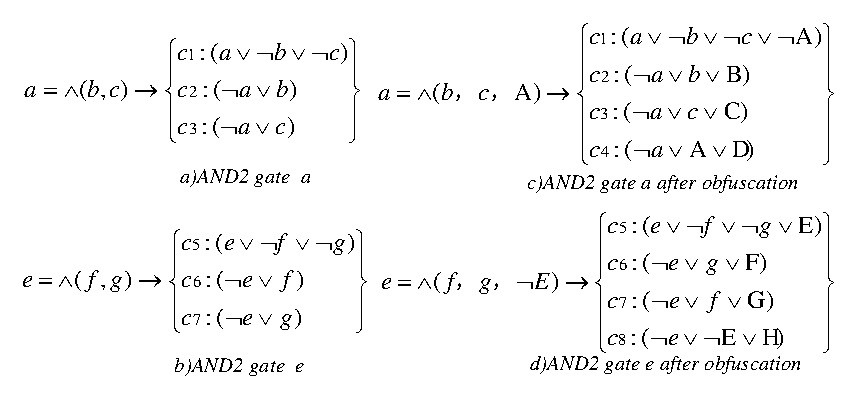
\includegraphics[width=8.2cm]{AND2-2}
\caption{CNF signature of $a$ and $e$ before and after obfuscation}
\label{fig_beforeafter}
\end{figure}

%Figure \ref{fig_beforeafter}a) and \ref{fig_beforeafter}b) shows the CNF signature and hyper-graph of two AND2 gate $a$ and $e$.
%While their CNF signature and hypergraph after obfuscating are shown in Figure \ref{fig_beforeafter}c) and \ref{fig_beforeafter}d).
Figure \ref{fig_beforeafter}a) and \ref{fig_beforeafter}b) shows the CNF signatures of two AND2 gates $a$ and $e$,
while their CNF signatures after obfuscation are shown in Figure \ref{fig_beforeafter}c) and \ref{fig_beforeafter}d).

There are three types of changes:
\begin{enumerate}
 \item
 The length of key clauses $c_1$ and $c_5$ are changed from 3 to 4,
this defeats structure detection techniques \cite{csFu} based on key clause oriented pattern matching;
 \item
CNF signatures of $a$ (characteristic clauses $c_1$-$c_3$) and $e$ (characteristic clauses $c_5$-$c_7$) are changed into different forms,
and there are new clauses added in formula, such as $c_4$ and $c_8$,
This defeats structure detection techniques\cite{csRoy} based on sub-graph isomorphic;
\item 
 By inserting proper literals in key clauses and generating new clause,
 CNF signature of gate $a$ is changed from AND2 to AND3,
shown in Figure \ref{fig_beforeafter}a) and \ref{fig_beforeafter}c).
Husk variable $A$,
which becomes an input variable of gate AND3,
is indistinguishable with $b$ and $c$,
which are original input variables of AND2.
This makes it impossible to distinguish gates AND2 and AND3.
\end{enumerate}

\subsubsection{Output Camouflage by over-approximating solution space}
According to Theorem \ref{SSOtheorem},
the solution space after SSO obfuscation is an over-approximated version of the original one.
That means, even SAT solver can't find out the real solution.
First, they can not tell real valuable variables from variables of Husks formula, 
which are meaningless to verification.
Second, they cannot tell if a satisfied solution means whether the original SAT problem is also satisfiable,
because some false solutions are produced by obfuscation.
Through overapproximation, We just turn an obvious Rare Events into a Camouflaged Rare Events, 
as anticipation in literature \cite{HV-grid} .

\subsection{Complexity}
\subsubsection{Obfuscation algorithm complexity}
Obfuscation is implemented in Algorithm \ref{algo_obs}.
The main procedure of Algorithm \ref{algo_obs} consists only one layer of loop,
but one of it sub-procedure $\mathbf{mark}$ (Algorithm \ref{algo_mark}) consists 4 layers of loop, 
and the runtimes of the 2 inner loops are bounded by length of clauses.
So the complexity of the obfuscation algorithm is $O(n^2)$.

\subsubsection{Solution recovery algorithm complexity}
Solution recovery is implemented in  Algorithm \ref{algo_map}, 
which only consists one layer of loop, 
its complexity is $O(n)$.
According to Theorem \ref{SSOtheorem}, result from SAT solver may consist false solution,
so Algorithm \ref{algo_map} may be run more than one time to get correct solution.
Since Algorithm \ref{algo_map} is of linear complexity,
it incurs minor impact on performance of SAT Solving.

\section{Related work}
\textbf{Secure Computation Outsourcing based on encryption:}
R. Gennaro et al.\cite{R.Gennaro} presented the concept of verifiable computation scheme,
which shows the secure computation outsourcing is viable in theory.
But the extremely high complexity of FHE operation and the pessimistic circuit sizes make it impractical.
Zvika et al.\cite{OBfuscationd-CNFs} constructed an obfuscated program for d-CNFs that preserves its functionality without revealing anything else.
The construction is based on a generic multi-linear group model and graded encoding schemes,
along with randomizing sub-assignments to enforce input consistency.
But the scheme incurs large overhead caused by their fundamental primitives.

\textbf{Secure Computation Outsourcing based on disguising:}
For linear algebra algorithms,
Atallah et al. \cite{t19} multiplied data with random diagonal matrix before outsourcing.
and recovered results by reversible matrix operations.
Paper \cite{t20} discussed secure outsourcing of numerical and scientific computation,
by disguising with a set of problem dependent techniques.
C.Wang\cite{c.WANG} presented securely outsourcing linear programming(LP) in Cloud,
by explicitly decomposing LP computation into public LP solvers and private data,
and provide a practical mechanism which fulfills input/output privacy,
cheating resilience, and efficiency.

\textbf{Verifiable computation delegation:}
Verifiable computation delegation is the technique to enable
a computationally weak customer to verify the correctness of the delegated computation results
from a powerful but untrusted server without investing too much resources.
To prevent participants from keeping the rare events,
Du. et al. \cite{HV-grid} injected a number of chaff items into the workloads so as to confuse dishonest participants.
Golle et al. \cite{t32} proposed to insert some pre-computed results images of ringers
into the computation workload to defeat untrusted or lazy workers.
Szada et al. \cite{t33} extended the ringer scheme and propose methods
to deal with cheating detection.

\section{Experiments}
Algorithms presented in this paper are implemented in language $C$.
The experiments is conducted on a laptop with Intel Core(TM) i7-3667U CPU @ 2.00GHz, 8GB RAM.

We unroll circuits in ISCAS89 benchmark for 100 times and transform them into CNF formulas,
and generate Husks formula with variables number $vn=675$ and clauses number $cn=2309$,
and then obfuscate the CNF formula by transform 2 input gates into 3 input gates.
We use MiniSat as solver.

Table \ref{fig_exp} presents experiments result on benchmarks, meaning of parameters are listed below. \\
$~~$\textbf{vn/cn}:variable and clause number of CNF formula.\\
$~~$\textbf{Marked Gate}:number of gates being changed in obfuscation.\\
$~~$\textbf{Solve Times}:SAT Solver time before and after obfuscation.\\
$~~$\textbf{Obfuscation Times}:obfuscation time.\\
$~~$\textbf{Map Time}:solution recovery time.

Acccording to Algorithm \ref{algo_obs},
Obfusaction time is up to number of gates being changed, 
while solution recovery time is up to size of CNF formula,
experiments manifest the fact.
% Detailed information are listed in columns of \textbf{Marked~Gate}, \textbf{Obfuscation Times} and \textbf{Map~Times}.

As for Asymmetric Speedup\cite{c.WANG}, for more than 60 \% of circuits, the value is more than 260\%,
It indicates the necessity of outsourcing complex SAT solving.
But for some small size circuits, 
Asymmetric Speedup is less than 1. 
Especially for circuit s3384, 
since the obfuscation takes lots of time to transform 139860 gates, Asymmetric Speedup is only 5.22\%.
\begin{equation}
 Asymmetric~Speedup= \frac{Solving~Time}{Obfuscation~Times + Map~Time} 
\end{equation}

The experiments also show that overhead of SAT solving time, incurred by obfuscation, 
are different among circuits.
For more than 60 \% of circuits, overhead is less than 30\%; But for the other 40\% circuits, overhead exceed 100\%.

These facts remind us at least two things: 
First, since  obfuscation time is up to gates being changed, 
delicate obfuscation algorithm which change less gates but still can mislead adversary should be studied.
Second, since overhead on SAT solving incurred by obfuscation are different among circuit benchmarks, 
much more attention should be pay on the impact on solving time,  when designing obfuscation algorithm. 
%\begin{figure}
%\centering
%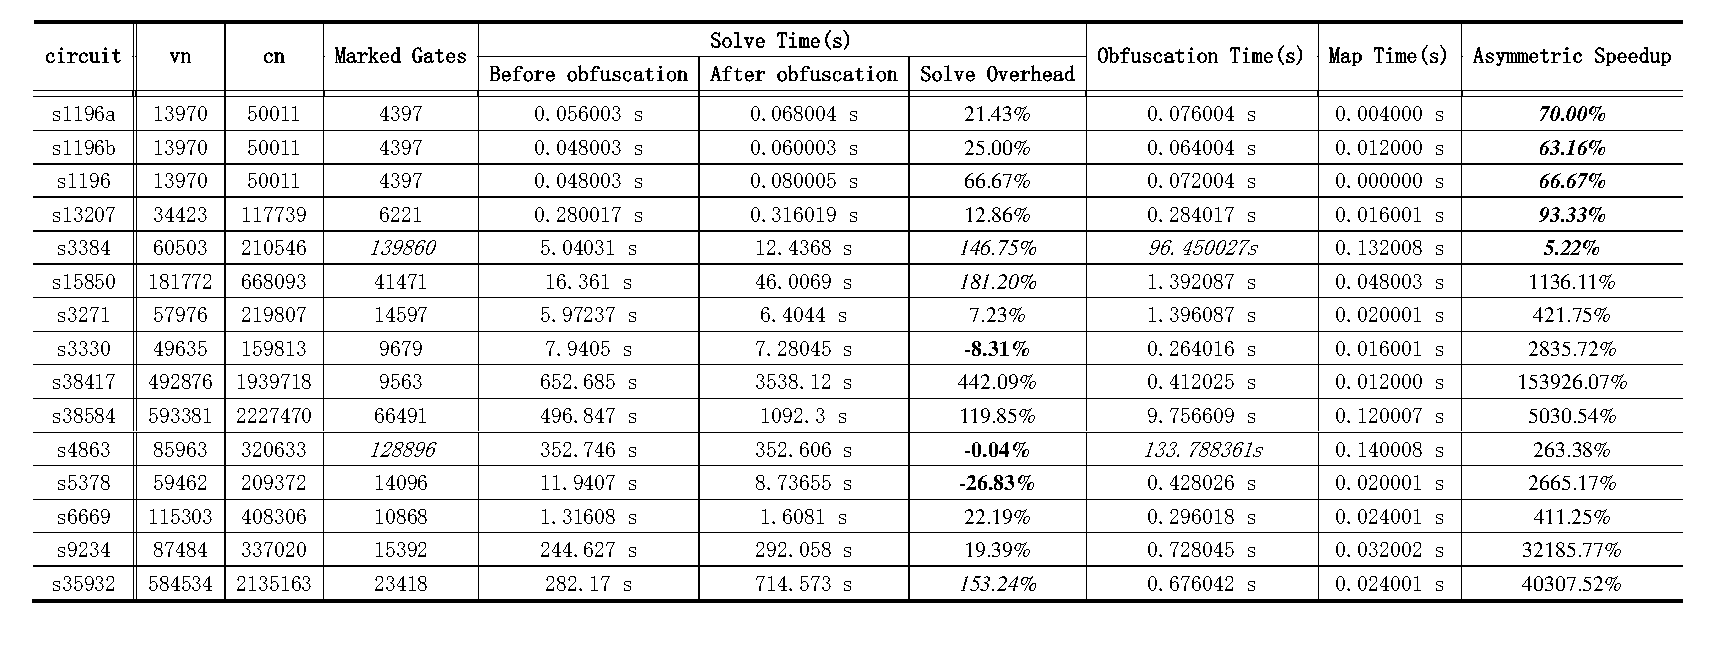
\includegraphics[width=16cm]{Experiment}
%\caption{Relationship between Runtime and Size of CNF formula}
%\label{fig_exp}
%\end{figure}

\begin{table*}
\caption{Runtime of CNF formula generated from different Circuit}
\centering
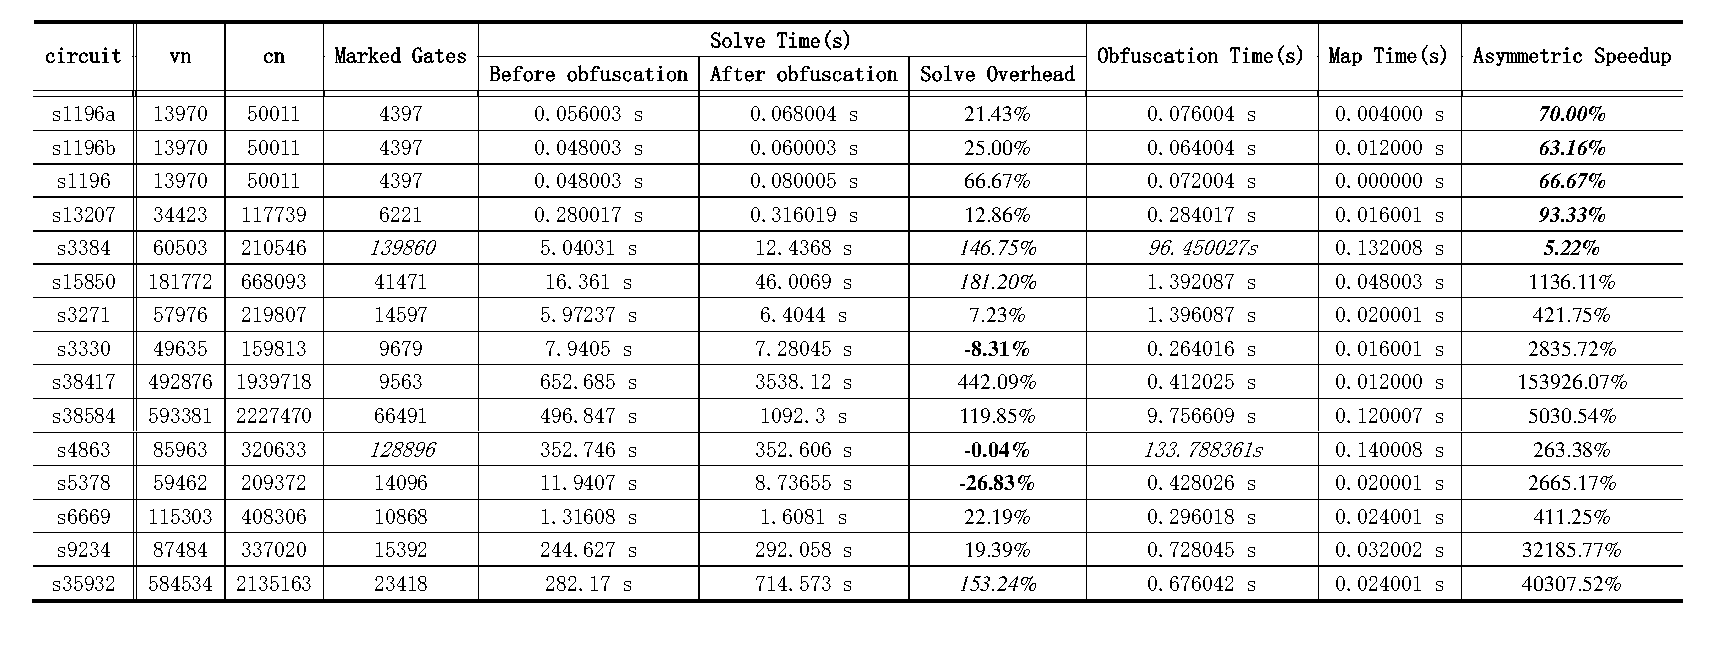
\includegraphics[width=18.2cm]{Experiment}
\label{fig_exp}
\end{table*}

\section{Conclusion}
This paper proposes a circuit aware  CNF obfuscation algorithm, 
that can prevent the confidential information from being recovered by adversary, 
when outsourcing SAT problem in Cloud or grid.
Theoretical analysis and experimental results show that algorithms can significantly change structure of CNF formula, 
with polynomial complexity and without narrowing down its solution space.

% An example of a floating figure using the graphicx package.
% Note that \label must occur AFTER (or within) \caption.
% For figures, \caption should occur after the \includegraphics.
% Note that IEEEtran v1.7 and later has special internal code that
% is designed to preserve the operation of \label within \caption
% even when the captionsoff option is in effect. However, because
% of issues like this, it may be the safest practice to put all your
% \label just after \caption rather than within \caption{}.
%
% Reminder: the "draftcls" or "draftclsnofoot", not "draft", class
% option should be used if it is desired that the figures are to be
% displayed while in draft mode.
%
%\begin{figure}[!t]
%\centering
%\includegraphics[width=2.5in]{myfigure}
% where an .eps filename suffix will be assumed under latex,
% and a .pdf suffix will be assumed for pdflatex; or what has been declared
% via \DeclareGraphicsExtensions.
%\caption{Simulation Results}
%\label{fig_sim}
%\end{figure}

% Note that IEEE typically puts floats only at the top, even when this
% results in a large percentage of a column being occupied by floats.


% An example of a double column floating figure using two subfigures.
% (The subfig.sty package must be loaded for this to work.)
% The subfigure \label commands are set within each subfloat command, the
% \label for the overall figure must come after \caption.
% \hfil must be used as a separator to get equal spacing.
% The subfigure.sty package works much the same way, except \subfigure is
% used instead of \subfloat.
%
%\begin{figure*}[!t]
%\centerline{\subfloat[Case I]\includegraphics[width=2.5in]{subfigcase1}%
%\label{fig_first_case}}
%\hfil
%\subfloat[Case II]{\includegraphics[width=2.5in]{subfigcase2}%
%\label{fig_second_case}}}
%\caption{Simulation results}
%\label{fig_sim}
%\end{figure*}
%
% Note that often IEEE papers with subfigures do not employ subfigure
% captions (using the optional argument to \subfloat), but instead will
% reference/describe all of them (a), (b), etc., within the main caption.


% An example of a floating table. Note that, for IEEE style tables, the
% \caption command should come BEFORE the table. Table text will default to
% \footnotesize as IEEE normally uses this smaller font for tables.
% The \label must come after \caption as always.
%
%\begin{table}[!t]
%% increase table row spacing, adjust to taste
%\renewcommand{\arraystretch}{1.3}
% if using array.sty, it might be a good idea to tweak the value of
% \extrarowheight as needed to properly center the text within the cells
%\caption{An Example of a Table}
%\label{table_example}
%\centering
%% Some packages, such as MDW tools, offer better commands for making tables
%% than the plain LaTeX2e tabular which is used here.
%\begin{tabular}{|c||c|}
%\hline
%One & Two\\
%\hline
%Three & Four\\
%\hline
%\end{tabular}
%\end{table}


% Note that IEEE does not put floats in the very first column - or typically
% anywhere on the first page for that matter. Also, in-text middle ("here")
% positioning is not used. Most IEEE journals/conferences use top floats
% exclusively. Note that, LaTeX2e, unlike IEEE journals/conferences, places
% footnotes above bottom floats. This can be corrected via the \fnbelowfloat
% command of the stfloats package.


%
%\section{Conclusion}
%The conclusion goes here.




% conference papers do not normally have an appendix


% use section* for acknowledgement
\section*{Acknowledgment}
This work was funded by projects 61070132 and 61133007 supported by National Natural Science Foundation of China.

% The authors would like to thank...





% trigger a \newpage just before the given reference
% number - used to balance the columns on the last page
% adjust value as needed - may need to be readjusted if
% the document is modified later
%\IEEEtriggeratref{8}
% The "triggered" command can be changed if desired:
%\IEEEtriggercmd{\enlargethispage{-5in}}

% references section

% can use a bibliography generated by BibTeX as a .bbl file
% BibTeX documentation can be easily obtained at:
% http://www.ctan.org/tex-archive/biblio/bibtex/contrib/doc/
% The IEEEtran BibTeX style support page is at:
% http://www.michaelshell.org/tex/ieeetran/bibtex/
%\bibliographystyle{IEEEtran}
% argument is your BibTeX string definitions and bibliography database(s)
%\bibliography{IEEEabrv,../bib/paper}
%
% <OR> manually copy in the resultant .bbl file
% set second argument of \begin to the number of references
% (used to reserve space for the reference number labels box)
\begin{thebibliography}{26}

\bibitem{SATtheory} 
M. Davis, H. Putnam: A Computing Procedure for Quantification Theory. J. ACM 7(3): 201-215 (1960)
\bibitem{HardwareSAT}
G. Hachtel, F. Somenzi.
Logic synthesis and verification algorithms. Springer 2006: I-XXIII, 1-564.
\bibitem{softwareSAT}
E. Clarke, O. Grumberg, S. Jha, Y. Lu, Helmut Veith: Counterexample-Guided Abstraction Refinement. CAV 2000: 154-169
\bibitem{cryptoSAT}
M. Soos, K. Nohl, C. Castelluccia: Extending SAT Solvers to Cryptographic Problems. SAT 2009: 244-257
\bibitem{Nordugrid}
A. Hyv\"arinen, T. Junttila, I. Niemel\"a: Grid-Based SAT Solving with Iterative Partitioning and Clause Learning. CP 2011: 385-399
\bibitem{Tseitin}
G. Tseitin.
On the complexity of derivation in propositional calculus. Studies in Constr. Math. and Math. Logic, 1968.
\bibitem{c.WANG}
C. Wang, K. Ren, J. Wang: Secure and practical outsourcing of linear programming in cloud computing. INFOCOM 2011: 820-828
\bibitem{csLiequivalency}
C. Li: Integrating Equivalency Reasoning into Davis-Putnam Procedure. AAAI/IAAI 2000: 291-296
\bibitem{csOstrowski}	
R. Ostrowski, \'E. Gr\'egoire, B. Mazure, L. Sais: Recovering and Exploiting Structural Knowledge from CNF Formulas. CP 2002: 185-199
\bibitem{csRoy}
J. Roy, I. Markov,V. Bertacco:
Restoring Circuit Structure from SAT Instances. IWLS'04, pp. 361-368.
\bibitem{csFu}
Z. Fu, S. Malik: Extracting Logic Circuit Structure from Conjunctive Normal Form Descriptions. VLSI Design 2007: 37-42
\bibitem{Minisat}
MiniSat-SAT Algorithms and Applications Invited talk given by Niklas Sorensson at the CADE-20 workshop ESCAR.
http://minisat.se/Papers.html
\bibitem{AMI}
M. Balduzzi, J. Zaddach, D. Balzarotti, E. Kirda, S. Loureiro: A security analysis of amazon's elastic compute cloud service. SAC 2012: 1427-1434
\bibitem{InformationLeakageofCloud}	
T. Ristenpart, E. Tromer, H. Shacham, S. Savage: Hey, you, get off of my cloud: exploring information leakage in third-party compute clouds. CCS 2009: 199-212
\bibitem{microgenSAT}
D. Achlioptas, C. Gomes, H. Kautz, B. Selman: Generating Satisfiable Problem Instances. AAAI/IAAI 2000: 256-261
\bibitem{genSAT} 
M Jarvisalo. Equivalence checking hardware multiplier designs.
SAT Competition 2007 benchmark description.
\bibitem{OBfuscationd-CNFs}
Z. Brakerski, G. Rothblum: Black-box obfuscation for d-CNFs. ITCS 2014: 235-250
\bibitem{R.Gennaro}
R. Gennaro, C. Gentry, B. Parno: Non-interactive Verifiable Computing: Outsourcing Computation to Untrusted Workers. CRYPTO 2010: 465-482
\bibitem{HV-grid}
W. Du, M. Goodrich: Searching for High-Value Rare Events with Uncheatable Grid Computing. ACNS 2005: 122-137
\bibitem{t19}
M. Atallah, K. Pantazopoulos, J. Rice, E. Spafford: Secure outsourcing of scientific computations. Advances in Computers 54: 215-272 (2001)
\bibitem{t20}
M. Atallah, J. Li: Secure outsourcing of sequence comparisons . Int. J. Inf. Sec. 4(4): 277-287 (2005)
\bibitem{t32}	
P. Golle, I. Mironov: Uncheatable Distributed Computations. CT-RSA 2001: 425-440
\bibitem{t33}
D. Szajda, B. Lawson, J. Owen: Hardening Functions for Large Scale Distributed Computations. IEEE Symposium on Security and Privacy 2003: 216-224
\bibitem{CloudSMT}
Paralleling OpenSMT Towards Cloud Computing http://www.inf.usi.ch/urop-Tsitovich-2-127208.pdf
\bibitem{OneSpin}
Formal in the Cloud OneSpin: New Spin on Cloud Computing.http://www. eejournal.com/archives/articles/20130627-onespin/?printView=true
\bibitem{obfuscationBible}
X.S. Zhang, F.L. He and W.l. Zuo. Theory and Practice of Program Obfuscation.
Convergence and Hybrid Information Technologies, Book edited by: Marius Crisan, ISBN 978-953-307-068-1, pp. 426, March 2010, INTECH, Croatia.
\bibitem{Partition} 
G. Karypis, R. Aggarwal, V. Kumar, S. Shekhar: Multilevel Hypergraph Partitioning: Application in VLSI Domain. DAC 1997: 526-529
%  \bibitem{IEEEhowto:kopka}
% H.~Kopka and P.~W. Daly, \emph{A Guide to \LaTeX}, 3rd~ed.\hskip 1em plus
%   0.5em minus 0.4em\relax Harlow, England: Addison-Wesley, 1999.

\end{thebibliography}



% that's all folks
\end{document}


